\documentclass[11pt]{aghdpl}
% \documentclass[en,11pt]{aghdpl}  % praca w języku angielskim
\usepackage[polish]{babel}
%\usepackage[english]{babel}
\usepackage[utf8]{inputenc}

% dodatkowe pakiety
\usepackage{enumerate}
\usepackage{listings}
\lstloadlanguages{TeX}

\lstset{
  literate={ą}{{\k{a}}}1
           {ć}{{\'c}}1
           {ę}{{\k{e}}}1
           {ó}{{\'o}}1
           {ń}{{\'n}}1
           {ł}{{\l{}}}1
           {ś}{{\'s}}1
           {ź}{{\'z}}1
           {ż}{{\.z}}1
           {Ą}{{\k{A}}}1
           {Ć}{{\'C}}1
           {Ę}{{\k{E}}}1
           {Ó}{{\'O}}1
           {Ń}{{\'N}}1
           {Ł}{{\L{}}}1
           {Ś}{{\'S}}1
           {Ź}{{\'Z}}1
           {Ż}{{\.Z}}1
}

\let\cleardoublepage\clearpage

%---------------------------------------------------------------------------

\author{Aleksander Nowak, Konrad Oboza}
\shortauthor{A. Nowak, K. Oboza}

\titlePL{Budowa aplikacji www wspierającej tryb offline przy użyciu HTML5}
\titleEN{Building offline enabled web application with HTML5}

\shorttitlePL{Budowa aplikacji www wspierającej tryb offline przy użyciu HTML5} % skrócona wersja tytułu jeśli jest bardzo długi
\shorttitleEN{Building offline enabled web application with HTML5}

\thesistype{Praca dyplomowa magisterska}
%\thesistype{Master of Science Thesis}

\supervisor{dr inż. Paweł Skrzyński}
%\supervisor{Marcin Szpyrka PhD, DSc}

\degreeprogramme{Informatyka}
%\degreeprogramme{Computer Science}

\date{2014}

\department{Katedra Informatyki Stosowanej}
%\department{Department of Applied Computer Science}

\faculty{Wydział Elektrotechniki, Automatyki,\protect\\[-1mm] Informatyki i Inżynierii Biomedycznej}
%\faculty{Faculty of Electrical Engineering, Automatics, Computer Science and Biomedical Engineering}

\acknowledgements{Składamy serdeczne podziękowania Panu dr ~Pawłowi Skrzyńskiemu za cenne wskazówki i pomoc w trakcie pisania pracy.}

\setlength{\cftsecnumwidth}{10mm}

%---------------------------------------------------------------------------
\setcounter{secnumdepth}{4}

\begin{document}

\titlepages
\setcounter{tocdepth}{3}
\tableofcontents
\clearpage

\chapter{Wstęp}
\label{cha:wstep}

Pozycja sieci Internet jako podstawowego i powszechnego medium komunikacyjnego jest niezachwiana od momentu jej powstania. Obecnie niemal wszystkie aplikacje dokonują synchronizacji za pomocą protokołów internetowych bez względu na platformę, na którą są przeznaczone. Dynamicznie rozwijające się standardy związane z protokołem HTTP (Hypertext Transfer Protocol) czyniące przeglądanie zasobów globalnej sieci łatwym i intuicyjnym za pośrednictwem każdego rodzaju urządzenia, potężne rozwiązania chmurowe oferujące platformy (PaaS), infrastruktury (IaaS) lub oprogramowanie (SaaS) jako usługi, czy szybka i przenośna bankowość elektroniczna to wybrane powody niesłabnącego zainteresowania rozwiązaniami internetowymi.

Tendencje rozwoju współczesnego oprogramowania warunkują konieczność znalezienia rozwiązania w sytuacjach braku dostępu do sieci Internet. Obejmuje ono metody przechowywania danych lokalnie z użyciem przeglądarki internetowej, sposoby ich replikacji i synchronizacji oraz detekcję połączenia.

Niniejsza praca dokonuje przeglądu wiodących metod lokalnego gromadzenia i przetwarzania danych użytkownika oraz obejmuje stworzenie aplikacji umożliwiającej pracę w trybach online oraz offline wraz z pełną synchronizacją danych pomiędzy klientem a serwerem wraz z bazą danych.

Postaramy się ustalić które z nowoczesnych technologii najlepiej radzą sobie z zachowaniem integralności w razie braku dostępu do sieci Internet.

Struktura niniejszej pracy jest następująca. Rozdział 1 przedstawia koncepcję i cele projektu. W rozdziale 2 dokonano analizy wymagań składowych projektu i przedstawiono wykorzystane technologie oraz paradygmaty. Rozdział 3 przedstawia założenia projektowe poszczególnych komponentów wraz z objaśnieniem wykorzystanych algorytmów. Rozdział 4 poświęcony jest przedstawieniu szczegółów implementacji. W rozdziale 5 zamieszczono krótką instrukcję instalacji i obsługi aplikacji. Rozdział 6 stanowi podsumowanie osiągniętych rezultatów.

\section{Cel pracy}
\label{sec:celPracy}

Celem niniejszej pracy jest przegląd metod lokalnego przechowywania danych z użyciem przeglądarki internetowej oraz projekt i implementacja aplikacji wspierającej tryby offline oraz online w oparciu o technologię HTML5.

\section{Dziedzina problemu}
\label{sec:dziedzinaProblemu}

Przeważająca część tworzonych obecnie aplikacji internetowych nie obsługuje sytuacji braku dostępu do sieci Internet. 

Dynamicznie rozwijające się przeglądarki oferują różne wsparcie dla technologii lokalnego przechowywania danych. Wspomniane mechanizmy stoją na zróżnicowanym poziomie standaryzacji, nierzadko procesy ich rozwijania zostają zawieszone. Różnią się one także stopniem złożoności obsługiwanych struktur danych.

Poważnym ograniczeniem są również limity przesyłanych danych na urządzeniach mobilnych a także koszty transmisji.

Utrudnienia związane z utrzymaniem stałego połączenia internetowego niosą ze sobą problemy z zachowaniem spójności i integralności synchronizowanych danych.

Istotną kwestią jest również dobór metod replikacji bazy danych celem minimalizacji liczby powstających konfliktów i ich poprawna obsługa.

\chapter{Analiza techniczna i analiza wymagań}
\label{cha:anaTechIAnaWym}

W rozdziale tym zostaną dokładnie przedstawione oraz porównane mechanizmy lokalnego przechowywania danych po stronie przeglądarki internetowej. Omówiony zostanie również problem dostępności aplikacji w trybie offline oraz używania aplikacji bez dostępnego połączenia internetowego i późniejszej synchronizacji danych.

Ponadto, w rozdziale zostaną przedstawione założenia systemu oraz wymagania które aplikacja powinna spełniać, a także narzędzia oraz technologie które pozwolą na wykonanie aplikacji zgodnie z założonymi wymaganiami.

%---------------------------------------------------------------------------

\section{Lokalne przechowywanie danych}
\label{sec:lokPrzechDanych}

Głównym wymogiem technicznym web aplikacji wspierającej tryb offline jest możlwość użytkowania jej bez konieczności połączenia z serwerem. Do realizacji tego wymogu niezbędne jest przechowywanie danych po stronie klienta - przeglądarki internetowej.

Przechowywanie danych po stronie klienta zawsze było mocną stroną aplikacji desktopowych. W przypadku web aplikacji, przez bardzo długi okres czasu ta funkcjonalność była ograniczona do tworzenia ciasteczek (cookie).

Cookie to niewielkie ilości danych każdorazowo przesyłane do serwera przy przeglądaniu danej witryny. Wsparcie przeglądarek dla plików cookie rozpoczęło się w 1995 roku i do drugiej dekady XXI wieku pliki cookie były jedyną szeroko wspieraną metodą przechowywania danych po stronie klienta. Pliki cookie posiadają kilka zasadniczych wad:


\begin{itemize}
\item Są przesyłane przy każdym zapytaniu HTTP kierowanym do serwera - niepotrzebnie zwiększenie transferu danych,
\item Pliki cookie są przesyłane do serwera niezależnie od użycia protokołu SSL - ryzyko podsłuchania ruchu sieciowego i wycieku danych,
\item Rozmiar pliku cookie nie może przekraczać 4KB - brak możliwości przechowywania większych ilości informacji.
\end{itemize}

W przypadku potrzeby uniknięcia ograniczeń cechujących ciasteczka, programista ma do wyboru kilka nowoczesnych metod przechowywania danych po stronie klienta, bazujących na specyfikacji HTML5: WebSQL, Web Storage, IndexedDB, File API. Metody te pozwalają na przechowywanie znacznie większych ilości danych oraz są manualnie przesyłane do serwera, co pozwala na optymalizację zapytań oraz większe bezpieczeństwo danych.

Jednym z kluczowych aspektów w przypadku wyboru metody lokalnego przechowywania danych w web aplikacji jest lista przeglądarek które wspierają daną metodę. O ile w przypadku plików cookie możemy mówić o pełnym wsparciu, o tyle poszczególne metody HTML5 posiadają zróżnicowane poziomy wsparcia zarówno na przeglądarkach desktopowych jak i mobilnych.

%---------------------------------------------------------------------------

\section{Mechanizmy lokalnego przechowywania danych}
\label{sec:mechLokPrzechDanych}

Aby budowa aplikacji www wspierającej tryb offline była możliwa, konieczny jest dobór odpowiedniego mechanizmu lokalnego przechowywania danych. Poniżej, pod względem funkcjonalności, łatwości użytkowania oraz wsparcia na konkretnych przeglądarkach, przeanalizowane zostały obecnie dostępne metody lokalnego przechowywania danych. Z uwagi na niezgodność z wymaganiami funkcjonalnymi aplikacji,  pliki cookie zostały pominięte w poniższej analizie.

%---------------------------------------------------------------------------

\subsection{HTML5 WebSQL Database}
\label{sec:html5WebSqlDatabase}

WebSQL Database jest mechanizmem, który do przechowywania, odczytu oraz aktualizacji danych po stronie klienta wykorzystuje strukturalny język zapytań SQL. Metoda działania mechanizmu bazuje na specyfikacji bazy SQLite. Mechanizm WebSQL posiada zarówno zalety przypisywane relacyjnym bazom danych oraz kilka zalet cechujących metody lokalnego zapisu danych:

\begin{itemize}
\item Transakcyjność,
\item Łatwość w utrzymaniu integralności danych,
\item Dobra wydajność w przypadku wyszukiwania zbioru elementów,
\item Szerokie spektrum zastosowań,
\item Rozmiar bazy danych ograniczony jedynie dostępną przestrzenią dyskową klienta,
\item Asynchroniczne wykonywanie zapytań - interfejs użytkownika nie jest blokowany do czasu zwróceniu rezultatu przez bazę danych.
\end{itemize}

Mechanizm WebSQL sprawdzi się dobrze w przypadku z góry zdefiniowanych struktur danych, które nie muszą być często zmieniane. W przypadku konieczności zmiany struktury danych, wymagane jest każdorazowe napisanie skryptu wykonującego zapytania SQL które pozwolą na aktualizację struktury bazy danych.

WebSQL jest metodą posiadającą umiarkowane wsparcie wśród popularnych przeglądarek internetowych. Poniżej znajduje się tabela przedstawiające wsparcie przeglądarek dla mechanizmu WebSQL zarówno na systemach desktopowych jak i mobilnych:

\begin{table}[h]
\centering
    \begin{tabular}{ | p{8cm} | p{6cm} | }
    \hline
    \textbf{Przeglądarka} & \textbf{Wsparcie (od wersji)} \\ \hline
	Google Chrome & 4.0
	\\ \hline
	Internet Explorer & brak
	\\ \hline
	Mozilla Firefox & brak
	\\ \hline
	Safari & 3.1
	\\ \hline
	Android Browser & 2.1
	\\ \hline
	Chrome for Android & 35.0
	\\ \hline
	iOS Safari & 3.2
	\\ \hline
    \end{tabular}
	\caption{Wsparcie mechanizmu WebSQL Database w przeglądarkach internetowych.}
\end{table}

Przy wyborze mechanizmu WebSQL jako metody przechowywania danych po stronie klienta należy wziąć pod uwagę fakt, że specyfikacja standardu nie jest dalej rozwijana. Z tego względu, przy wyborze tej technologii należy liczyć się z możliwością utraty wsparcia na przeglądarkach, które w chwili obecnej je zapewniają. Dodatkowo, przeglądarki które w tym momencie nie oferują wsparcia dla tego mechanizmu, nie dodadzą go przy premierze kolejnych ich wersji.

Biorąc pod uwagę powyższe informacje, użytkowanie aplikacji www bazującej na mechaniźmie WebSQL po aktualizacji przeglądarki do nowszej wersji może stać się niemożliwe. Stoi to w sprzeczności z wymaganiami funkcjonalnymi aplikacji, dlatego mechanizm ten nie zostanie wykorzystany przy budowie aplikacji wspierającej tryb offline.

\subsection{HTML5 Web Storage}
\label{sec:html5WebStorage}

HTML5 Web Storage, znany również jako DOM Storage, jest mechanizmem, który przechowuje dane w tablicy asocjacyjnej w której klucze oraz wartości są ciągami tekstowymi. W zależności od przeglądarki internetowej, maksymalny rozmiar danych możliwy do zapisu wynosi od 5 do 35 megabajtów danych.

Web Storage udostępnia dwa obszary składowania danych różniące się zasięgiem oraz cyklem życia:

\begin{itemize}
\item \emph{localStorage} - dane są dostępne we wszystkich oknach oraz kartach danej przeglądarki, dane nie są usuwane po zamknięciu przeglądarki,
\item \emph{sessionStorage} - dane dostępne w obrębie jednej karty przeglądarki, usuwane po jej zamknięciu.
\end{itemize}

Największymi zaletami mechanizmu Web Storage jest kompleksowe wsparcie na wszystkich obecnie popularnych przeglądarkach internetowych, jak również łatwość jego obsługi - pobranie wartości danego elementu następuje synchronicznie poprzez odwołanie się do globalnego obiektu localStorage lub sessionStorage wraz z podaniem w notacji tablicowej klucza - ciągu znakowego - identyfikującego dany element.

\begin{table}[h]
\centering
    \begin{tabular}{ | p{8cm} | p{6cm} | }
    \hline
    \textbf{Przeglądarka} & \textbf{Wsparcie (od wersji)} \\ \hline
	Google Chrome & 4.0
	\\ \hline
	Internet Explorer & 8.0
	\\ \hline
	Mozilla Firefox & 3.5
	\\ \hline
	Safari & 4.0
	\\ \hline
	Android Browser & 2.1
	\\ \hline
	Chrome for Android & 35.0
	\\ \hline
	iOS Safari & 3.2
	\\ \hline
    \end{tabular}
	\caption{Wsparcie mechanizmu Web Storage w przeglądarkach internetowych.}
\end{table}

Prostota mechanizmu Web Storage ma również swoje wady. Największą z nich jest brak możliwości przechowywania zaawansowanych struktur danych w formacie innym niż łańcuch znaków. W takim przypadku konieczna jest serializacja danych przy zapisie oraz ich deserializacja przy odczycie, co w przypadku dużych obiektów może doprowadzić do problemów z wydajnością.

Dużym ograniczeniem metody jest również brak możliwości efektywnego przeszukiwania danych oraz ich indeksowania. W większości przypadków prowadzi to do konieczności iteracji po wszystkich zdefiniowanych elementach. Synchroniczność zapytań oraz konieczność deserializacji otrzymanych danych skutecznie obniżają szybkość wyszukiwania, szczególnie w przypadku dużej ilości przechowywanych obiektów.

Zarówno konsorcjum W3C zajmujące się rozwojem standardu Web Storage, jak i firmy zajmujące się tworzeniem przeglądarek internetowych są zainteresowane umożliwieniem przechowywania bardziej zaawansowanych struktur danych. Pozwoliłoby to na efektywne zastosowanie Web Storage w przypadku złożonych obiektów. Biorąc pod uwagę cykl życia przeglądarek internetowych oraz średni czas potrzebny użytkownikowi na jej aktualizację, uzyskanie szerszego wsparcia dla tej aktualizacji może zająć kilka lat.

Mechanizm Web Storage posiada pełne wsparcie w obecnych klientach sieci www, jednak nie posiada on wydajnej metody przeszukiwania przechowywanych danych, przez co jego wykorzystanie przy budowie aplikacji www wspierającej tryb offline jest niezalecane na tym etapie rozwoju mechanizmu.

\subsection{HTML5 IndexedDB}
\label{sec:html5IndexedDB}

Indexed Database jest mechanizmem, który powstał na bazie Web Storage oraz WebSQL, łączy cechy obydwu specyfikacji. IndexedDB przechowuje obiekty języka JavaScript w magazynach obiektów (\emph{objectStores}) które są odpowiednikami tabel w relacyjnej bazie danych.

Każdy rekord przetrzymywany w magazynie musi posiadać unikalny klucz główny który może zostać zdefiniowany przez użytkowika lub, w przeciwnym wypadku, zostanie utworzony automatycznie. W celu optymalizacji przeszukiwania zbioru danych, IndexedDB umożliwia zdefiniowanie indeksu na dowolnym z atrybutów przechowywanych obiektów. Znacząco skraca to czas wyszukiwania oraz ilość potrzebnych do tego zasobów.

Podobnie jak w przypadku mechanizmu WebSQL, IndexedDB wykonuje zapytania asynchronicznie, pozwalając na interakcję użytkownika z aplikacją podczas wykonywania zapytań. Mechanizm wspiera również wersjonowanie bazy danych - w przypadku konieczności aktualizacji bazy do nowszej wersji wykonywane są zdefiniowane przez programistę instrukcje, które powinny zapewnić spójność poprzez aktualizację danych znajdujących się w poprzedniej wersji magazynów obiektów.

Ilość miejsca, jaka może zostać przeznaczona na zasoby przechowywane w IndexedDB jest nieograniczona. W przypadku przekroczenia granicznego rozmiaru bazy danych, indywidualnie ustalanego dla danej przeglądarki internetowej, użytkownik musi wyrazić zgodę na zniesienie ograniczenia ilości miejsca przeznaczonego na magazyny obiektów.

Indexed Database posiada dobre wsparcie wśród nowszych wersji popularnych przeglądarek internetowych.

\begin{table}[h]
\centering
    \begin{tabular}{ | p{8cm} | p{6cm} | }
    \hline
    \textbf{Przeglądarka} & \textbf{Wsparcie (od wersji)} \\ \hline
	Google Chrome & 23.0
	\\ \hline
	Internet Explorer & 10.0
	\\ \hline
	Mozilla Firefox & 10.0
	\\ \hline
	Safari & 8.0
	\\ \hline
	Android Browser & 4.4
	\\ \hline
	Chrome for Android & 35.0
	\\ \hline
	iOS Safari & 8.0
	\\ \hline
    \end{tabular}
	\caption{Wsparcie mechanizmu IndexedDB w przeglądarkach internetowych.}
\end{table}

IndexedDB łączy najlepsze funkcjonalności WebSQL oraz Web Storage. Biorąc pod uwagę dobre wsparcie wśród przeglądarkek, szybkie czasy wyszukiwania elementów przy użyciu indeksów oraz możliwość przechowywania obiektów bez konieczności ich serializacji, mechanizm ten spełnia wszystkie wymagania aplikacji www wspierającej tryb offline.

\subsection{HTML5 Filesystem API}
\label{sec:html5filesystemApi}

Filesystem API jest mechanizmem który umożliwia operacje na plikach znajdujących się w wydzielonej przestrzeni na dysku twardym użytkownika. Aby zapis na dysku był możliwy, użytkownik musi najpierw upoważnić do tego aplikację, co odbywa się poprzez zaakceptowanie okna dialogowego wyświetlającego żądanie przechowywania konkretnej ilości danych, jaką dana aplikacja zamierza wykorzystać.

Lista funkcji udostępnianych przez Filesystem API obejmuje zarówno operacje na plikach - zapis, odczyt pliku, odczyt metadanych pliku, kopia do wskazanej lokacji, oraz narzędzia do tworzenia drzewa katalogów oraz ich przeszukiwania. Pliki przechowywane na wydzielonej przestrzeni dyskowej mogą później zostać osadzone jako elementy strony www - jedna z metod Filesystem API zwraca pełny adres URL do danego zasobu.

Pomimo wysokiej użyteczności mechanizmu Filesystem API, wsparcie przeglądarkek ograniczna się do Google Chrome oraz Chrome for Android. W związku z niskim zainteresowaniem innych firm zajmujących się rozwijaniem przeglądarek internetowych, organizacja W3C zawiesiła prace nad tym standardem.

\begin{table}[h]
\centering
    \begin{tabular}{ | p{8cm} | p{6cm} | }
    \hline
    \textbf{Przeglądarka} & \textbf{Wsparcie (od wersji)} \\ \hline
	Google Chrome & 12.0
	\\ \hline
	Internet Explorer & brak
	\\ \hline
	Mozilla Firefox & brak
	\\ \hline
	Safari & brak
	\\ \hline
	Android Browser & brak
	\\ \hline
	Chrome for Android & 35.0
	\\ \hline
	iOS Safari & brak
	\\ \hline
    \end{tabular}
	\caption{Wsparcie mechanizmu Filesystem API w przeglądarkach internetowych.}
\end{table}

Filesystem API jest bardzo dobrym rozwiązaniem dla aplikacji, które wymagają przechowywania dużej ilości zasobów - plików audio, wideo, zdjęć, dokumentów. W przypadku aplikacji które przechowują dane strukturalne, metody WebSQL oraz IndexedDB okażą się dużo bardziej efektywne. Ze względu na niskie wsparcie przeglądarek oraz zawieszenie prac nad rozwojem specyfikacji Filesystem, mechanizm ten nie spełnia wymagań stawianych aplikacji www wspierającej tryb offline.

\section{Aplikacje webowe trybu offline}
\label{sec:appWebOff}

Tryb offline (w wolnym tłumaczeniu: "bez dostępu do sieci Internet") nie był dotychczas kojarzony z przeglądarkami internetowymi - programami z definicji służącymi do przeglądania zasobów WWW (\emph{World Wide Web}). Aplikacje pracujące w tym trybie mogły być wywoływane jedynie poprzez ścieżkę rozpoczynającą się od \textbf{file://} i odwoływać się do danych znajdujących się na dysku twardym, flash lub płycie CD/DVD. Przykładem mogą być prezentacje korzystające z przeglądarki celem uruchomienia animacji napisanych za pomocą języka JavaScript.

Tryb offline pojawia się obecnie również w tak zwanych \textbf{Single-page applications}. Ich działanie polega na wykorzystaniu funkcji przeglądarki internetowej do interakcji z użytkownikiem i zapisania danych lokalnie. Przykład stanowić może TiddlyWiki - osobiste wiki umożliwiające tworzenie i edytowanie treści poprzez uruchomienie pojedynczej strony w przeglądarce bez dostępu do sieci Internet. Cel ten może zostać osiągnięty dzięki dobrodziejstwom oferowanym przez specyfikację HTML5.

Dochodzimy wreszcie do aplikacji wspierających zarówno tryb offline jak i online. Koncepcja ta wykorzystana jest w niniejszej pracy.

Często zasadność tworzenia aplikacji działającej bez dostępu do sieci jest poddawana w wątpliwość. Ogólnodostępność Internetu sprawia, że nawiązanie połączenia nie stanowi obecnie żadnej trudności.

Pomimo prawdziwości powyższego stwierdzenia należy brać pod uwagę względy oszczędnościowe i lokalizacyjne. Mobilność a co za tym idzie ciągła synchronizacja aplikacji zainstalowanych na urządzeniach przenośnych powoduje wzrost zużycia energii. Ponadto nadal istnieją miejsca, gdzie dostęp do sieci Internet jest zabroniony (pokład samolotu) znacząco utrudniony lub nawet niemożliwy.

Poniżej przedstawimy główne prawidłowości działania trybu offline przez pryzmat przeglądarek internetowych.

\subsection{Pamięć cache}
\label{sec:pamiecCache}

Pamięć podręczna przeglądarki (ang. \emph{cache}) obejmuje miejsce na dysku twardym przeznaczone do przechowywania odwiedzonych stron WWW lub ich fragmentów. Najczęściej dotyczy to arkuszy stylów CSS, grafik a także skryptów w języku JavaScript. Wyróżniamy dwa główne powody stosowania cache-owania:

\begin{itemize}
\item \textbf{redukcja czasu dostępu do zasobów:} pamięć cache jest znacznie “bliżej” klienta, niż serwer oryginalny, dzięki czemu w krótszym czasie uzyskiwany jest dostęp do konkretnego zasobu i jego prezentacja,
\item \textbf{redukcja ruchu sieciowego:} przechowywane w pamięci podręcznej zasoby mogą zostać użyte ponownie, co zmniejsza rozmiar pasma niezbędnego do uzyskania dostępu i oszczędza koszty ponoszone przez użytkownika.
\end{itemize}

Pamięć cache dokonuje aktualizacji przechowywanych treści najczęściej raz na sesję (za rozpoczęcie sesji przyjmujemy uruchomienie przeglądarki) tak, by użytkownik był na bieżąco ze zmianami treści. Poniżej przedstawiono ogólne zasady działania Web Cache:

\begin{enumerate}
\item Działaniem cache sterują nagłówki HTTP. Użytkownik może zdecydować między innymi o czasie przechowywania "świeżej" porcji danych w pamięci, ich dostępności (private/public) lub nawet o wyłączeniu cache-owania danych.
\item Żądania uwierzytelnienia lub żądania zabezpieczone (np. HTTPS) nie są cache-owane.
\item Reprezentacja danych w cache jest uważana za "świeżą" (nie musi być sprawdzana z wersją danych na serwerze oryginalnym), jeśli ustawiono nagłówek HTTP odpowiadający za czas życia danych lub jeśli dane były cache-owane niedawno.
\item Jeśli dane są nieaktualne do serwera zostanie wysłane zapytanie o walidację.
\item W sytuacji utraty połączenia internetowego pamięć cache może wysyłać dane bez weryfikacji ich z danymi pochodzącymi z oryginalnego serwera.
\end{enumerate}

W przypadku braku dostępu do nagłówków HTTP możliwa jest edycja ustawień pamięci cache za pomocą znaczników \textbf{meta} zawartych w sekcji head definicji dokumentu HTML.

Proces zapisywania w pamięci podręcznej jest w dużej mierze zautomatyzowany i związany z wyświetleniem witryny. Należy rozgraniczyć na czym polegać, w kontekście projektu, będzie przechowywanie lokalne.

Użytkownik manualnie wywoła proces zapisu danych wykonując akcje na interfejsie aplikacji jak na przykład dodanie/edycja/usunięcie wydarzenia, edycja ustawień etc. Bez ingerencji dane nie trafią do pamięci podręcznej w odróżnieniu od cache-owania wykonywanego automatycznie podczas wyświetlenia dokumentu HTML.

\subsection{Detekcja połączenia sieciowego}
\label{sec:detPolSieciowego}

Wymogiem działania aplikacji jest automatyczna detekcja połączenia internetowego i przejście do trybu online/offline. Jest to spowodowane koniecznością uruchomienia zapisu lokalnego lub synchronizacji danych do serwera aplikacji.

Specyfikacja HTML5 oferuje różne mechanizmy wykrywania połączenia sieciowego. Różnią się one poziomem wsparcia w przeglądarkach.

Jednym z nich jest skorzystanie z tzw. Obserwatora Zdarzeń (\emph{EventListener}). HTML5 udostępnia obserwatory \textbf{online} oraz \textbf{offline}.

Połączenie internetowe może także zostać zweryfikowane za pomocą obiektu \textbf{XMLHttpRequest (XHR)}. Jest to obiekt języków skryptowych (jak np. JavaScript) umożliwiający wykonanie żądań po załadowaniu się dokumentu HTML. Są one realizowane asynchronicznie (w tle) i nie przerywają interakcji użytkownika ze stroną. Badanie dostępu do Internetu ogranicza się do sprawdzenia odpowiedzi z serwera.

Biblioteką również wykorzystującą technologię AJAX (\emph{Asynchronous JavaScript and XML}) w detekcji połączenia jest Offline.js. Umożliwia ona wykrycie utraconego połączenia oraz ponowne wykonanie żądań, które w wyniku owej utraty nie doszły do skutku. Dodatkowo oferuje szablony służące do wyświetlenia odpowiednich informacji dla użytkownika.

Szczegóły zastosowanych mechanizmów zostaną omówione w rozdziałach poświęconych projektowi i implementacji systemu.

\section{Replikacja i synchronizacja danych}
\label{sec:repIsynchDanych}

Niezbędnym elementem aplikacji www wspierającej tryb offline jest mechanizm  przechowywania danych po stronie klienta. W momencie zerwania połączenia sieciowego  i utraty komunikacji z serwerem, użytkownik powinien posiadać lokalną replikę danych znajdujących się na serwerze. W replice tej powinny zostać zapisane wszystkie wykonane przez niego akcje.

W chwili uzyskania ponownego dostępu do sieci, dane przechowywane w lokalnej bazie danych muszą zostać zsynchronizowane z danymi znajdującymi się na serwerze aby możliwa była ich dalsza propagacja do pozostałych urządzeń z których korzysta dany użytkownik.

Aby aplikacja była w stanie wykonać powyższe zadania, konieczne jest dobór odpowiedniej metody replikacji oraz sychronizacji danych, która pozwoli na stabilne i spójne działanie aplikacji, niezależnie od akcji wykonywanych przez użytkownika oraz stanu połączenia sieciowego.

\subsection{Podstawowe pojęcia}
\label{sec:podstPojecia}

\textbf{Replikacja danych} jest procesem w którym operacje wykonane na danej instacji bazy danych są powielane na pozostałych instancjach objętych mechanizmem replikacji. Głównym celem replikacji jest zwiększenie dostępności oraz szybkości usług sieciowych. Dostępność jest zwiększona poprzez możliowść dostępu do danych w przypadku gdy dostępna jest tylko część replik. Szybkość usług jest zwiększona poprzez dostęp użytkowników do najbliższej, względem ich lokacji, repliki. Prowadzi to do mniejszego opóźnienia sieciowego oraz rozłożenia obciążenia pomiędzy poszczególne repliki wchodzące w skład systemu.

W przypadku aplikacji www wspierających tryb offline mamy do czynienia z przypadkiem, gdy mechanizm lokalnego przechowywania danych obsługiwany przez przeglądarkę użytkownika staje się jedną z replik danych.

\textbf{Transakcją} nazywamy zbiór operacji na bazie danych, które tworzą pewną całość. Aby zmiany wprowadzone przez transakcję zostały zapisane w bazie danych, wszystkie operacje składające się na transakcję muszą zostać poprawnie wykonane. Transakcje powinny spełniać warunki opisane w zasadach ACID (Atomowość, Spójność, Izolacja, Trwałość):

\begin{itemize}
\item Atomowość - w przypadku niepowodzenia przynajmniej jedenej operacji wchodzącej w skład transakcji cała transakcja jest anulowana, pozostawiając dane w niezmienionej formie,
\item Spójność - przed, w trakcie oraz po wykonaniu transakcji system pozostaje w spójnym stanie i nie naruszona zasady integralności danych,
\item Izolacja - w przypadku wielu transakcji wykonywanych współbieżnie, zmiany dokonywane przez poszczególne transakcje są widoczne tylko i wyłącznie z perspektywy danej transakcji.
\item Trwałość - w przypadku awarii, dane wszystkich transakcji które zostały zatwierdzone są zapisane w systemie i będą dostępne po ponownym jego uruchomieniu.
\end{itemize}

\textbf{Szeregowalność} jest pożądaną własnością systemów bazodanowych, która umożliwia zarządzanie operacjami wykonywanymi współbieżnie na bazie danych w taki sposób, aby wyeliminować niepożądane interakcje między nimi. Szeregowalność zapewnia taki sam stan końcowy danych po współbieżnym wykonaniu danych transakcji, jak i po wykonaniu tych transakcji szeregowo.

\textbf{Zakleszczenie} jest zdarzeniem, które zachodzi w sytuacji gdy dwa procesy, każdy z nich wykonujący transakcję, modyfikują wspólny zbiór rekordów w odwrotnej kolejności Prowadzi to do sytuacji, w której każdy z procesów czeka na zakończenie przeciwnego, co w przypadku zakleszczenia nie następuje. System zarządzania bazą danych odpowiada za wykrywanie zakleszczeń i ich rozwiązywanie, zazwyczaj przez anulowanie jednej z transakcji.

\subsection{Klasyfikacja technik replikacji}
\label{sec:klasTechReplik}

Istnieje wiele technik replikacji które pozwalają na skuteczną oraz stabilną pracę rozproszonych systemów bazodanowych. Główne cechy replikacji które muszą zostać określone to:

\begin{itemize}
\item zakres replikowanych danych,
\item sposób sychronizacji pomiędzy węzłami,
\item poziom dostępu do danych w zależności od statusu repliki.
\end{itemize}

Poniżej przedstawione zostały klasyfikacje które pomagą określić typ replikacji, który oferuje najlepszą funkcjonalność w przypadku aplikacji www wspierających tryb offline.

\setlength{\parskip}{10pt plus 1pt minus 1pt}
\textbf{Replikacja całościowa - Replikacja częściowa}
\setlength{\parskip}{10pt plus 1pt minus 1pt}

Replikacja całościowa zapewnia dostępność pełnej kopii danych na wszystkich węzłach wchodzących w skład systemu.

Replikacja częściowa pozwala na wybór danych, które będą replikowane, przy czym zbiór danych podlegających replikacji jest określany indywidualnie dla każdego węzła wchodzącego w skład systemu. Replikacja częściowa może dzielić zbiór danych na dwa sposoby:

\begin{itemize}
\item horyzontalnie - z danej tabeli wybrany jest zbiór wierszy zawierający wszystkie wartości dla kolumn zdefiniowanych w tej tabeli.
\item wertykalnie - z danej dabeli wybrany jest zbiór kolumn, których wartości dla każdego wiersza są replikowane.
\end{itemize}

\setlength{\parskip}{10pt plus 1pt minus 1pt}
\textbf{Replikacja synchroniczna - Replikacja asynchroniczna}
\setlength{\parskip}{10pt plus 1pt minus 1pt}

Replikacja synchroniczna, tzw. "gorliwa", stara się utrzymać zsynchronizowane dane pomiędzy wszystkimi węzłami wchodzącymi w skład systemu. W przypadku replikacji synchronicznej, w skład transakcji wchodzi propagacja danych do wszystkich węzłów - w przypadku wystąpienia konfliktu transakcja jest anulowana. Zapewnia to ochronę przed możliwymi niespójnościami w bazie danych, jednak ryzyko zakleszczenia znacząco wzrasta wraz ze wzrostem liczby transakcji.

Replikacja asynchroniczna, tzn. "leniwa", pozwala na niezależne wykonywanie transakcji na każdym z węzłów. Po wykonaniu transakcji na jednym z węzłów, dane są asynchronicznie propagowane do pozostałych węzłów. Replikacja leniwa nie wymaga wysokiej dostępności węzłów, jednak może prowadzić do konfliktów.

Przykładem obrazującym różnicę pomiędzy replikacją leniwą a replikacją gorliwą może być próba wykonania dwóch przelewów z dwóch różnych węzłów objętych replikacją, gdzie obciążenie rachunku przekracza dostępne saldo. W przypadku replikacji gorliwej, pierwsza z transakcji zostanie wykonana pomyślnie, druga zwróci komunikat błędu. W przypadku replikacji leniwej, obie transakcje zakończą się sukcesem, jednak w fazie synchronizacji danych dojdzie do konfliktu, który będzie musiał zostać obsłużony.

\setlength{\parskip}{10pt plus 1pt minus 1pt}
\textbf{Replikacja pesymistyczna - Replikacja optymistyczna}
\setlength{\parskip}{10pt plus 1pt minus 1pt}

Replikacja pesymistyczna zakłada, że stan obiektów przechowywanych w każdym węźle jest identyczny oraz aktualny. W celu uniknięcia konfliktów, w przypadku nieaktualnego stanu danych w węźle, dostęp do danych jest blokowany.

Replikacja optymistyczna nie ogranicza w żaden sposób dostępu do danych, niezależnie od stanu w którym znajduje się replika. Każda z replik przechowuje historię wykonanych transakcji. Ze względu na niezależne wykonywanie transakcji na każdym węźle, w momencie synchronizacji system jest narażony na możliwe konflikty danych. Prowadzi to do konieczności modyfikacji części transakcji i ponownego ich wykonania, co może skutkować innym stanem bazy danych po zakończeniu synchronizacji.

\subsection{Replikacja danych w aplikacji www wspierającej tryb offline}
\label{sec:replDanWAplWWWWspTrybOffline}

Aplikacja www wspierająca tryb offline powinna minimalizować ilość danych przesyłanych pomiędzy poszczególnymi węzłami systemu. Ze względu na prywatność danych, lokalna replika powinna posiadać wyłącznie dane powiązane z konkretnym, zalogowanym w danym momencie do aplikacji, użytkownikiem. Dodatkowo, uwzględniając coraz większą aktywność użytkowników korzystających z urządzeń mobilnych, aplikacja powinna ograniczyć ilość przesyłanych danych do minimum. Z tego względu, replikacja częściowa jest w tym przypadku znacznie lepszym wyborem od replikacji całościowej.

Z uwagi na wymagania aplikacji www oraz nacisk położony na pełną jej funkcjonalność w trybie offline, synchronizacja danych pomiędzy węzłami powinna odbywać się w sposób "leniwy". Przechowywanie danych w lokalnej replice oraz późniejsza asynchroniczna wymiana informacji pomiędzy węzłami powinna zapewnić bardzo płynną interakcję z interfejsem użytkownika, co jest jednym z wymagań aplikacji.  W przypadku użytkowników posiadających repliki danych na wielu urządzeniach które przez większość czasu są fizycznie wyłączone lub nie posiadają dostępu do sieci, zastosowanie replikacji "gorliwej" nie byłoby możliwe.

Użytkownik korzystający z aplikacji na urządzeniu mobilnym może znaleźć się w rejonie o słabym zasięgu sieci telefonicznej. W celu oszczędności energii oraz minimalizacji transferu danych przez sieć mobilną, użytkownik może wyłączyć mobilny transfer danych. W przypadku zastosowania replikacji pesymistycznej, uniemożliwiłoby to komunikację z lokalną repliką danych ze względu na nieosiągalność pozostałych węzłów. Z tego względu w aplikacji www wspierającej tryb offline powinna zostać zastosowana replikacja optymistyczna.

Zastosowanie replikacji posiadającej powyższe cechy może doprowadzić do sytuacji, w których podczas procesu synchronizacji wystąpi konflikt transakcji. Aplikacja powinna posiadać wewnętrzne algorytmy które obsłużą takie sytuacje, zaś w przypadku braku możliwości programatycznej obsługi, użytkownik powinien zostać poinformowany o konflikcie oraz o możliwościach jego rozwiązania.

\section{Analiza wymagań}
\label{sec:analizaWymagan}

Tworzony system służy do zarządzania wydarzeniami użytkownika. Zorganizowany jest on w formie interaktywnego kalendarza. Główną zaletą aplikacji jest pełne wsparcie zarówno trybu online jak i offline co uniezależnia ją od stałego dostępu do sieci Internet. Poniższa analiza sugeruje jedynie możliwe zastosowanie systemu zgodnie z jego
pierwotnymi założeniami, aczkolwiek nie wyklucza innej aktywności. Szczegółowy opis możliwości systemu zawarty jest w treści poniższych podrozdziałów.

\subsection{Wymagania funkcjonalne}
\label{sec:wymFunkcj}

Zadaniem aplikacji jest dodawanie, edycja oraz usuwanie wydarzeń. Przez wydarzenie rozumiemy notatkę składającą się z nazwy, czasu trwania oraz treści. Dzięki zaimplementowanemu systemowi autentykacji każdy użytkownik posiada konto, co jednoznacznie identyfikuje wprowadzone przez niego dane. Ponadto użytkownik ma do dyspozycji system powiadomień o nadchodzących wydarzeniach. Jest on w pełni konfigurowalny.

Podane akcje mogą być wykonywane zarówno w trybie offline jak i przy aktywnym połączeniu z siecią Internet. Dane gromadzone lokalnie zostają zsynchronizowane z tymi obecnymi w bazie danych serwera aplikacji w momencie wykrycia połączenia. Sam proces synchronizacji może zakończyć się niepowodzeniem, co zostanie obsłużone automatycznie przez zaimplementowane algorytmy lub manualnie, po uprzednim poinformowaniu użytkownika o problemie.

Krytycznym wymaganiem funkcjonalnym systemu jest zapewnienie integralności danych i zapewnienie ciągłości transakcji pomimo problemów z połączeniem sieciowym. Przejście pomiędzy trybami online/offline powinno być płynne i nie wpływać negatywnie na wydajność interfejsu użytkownika.

Z uwagi na zastosowanie optymistycznej replikacji bazy danych należy zwrócić baczną uwagę na możliwość wystąpienia konfliktów pomiędzy żądaniami i ich obsługę.

\subsection{Wymagania niefunkcjonalne}
\label{sec:wymNieFunkcj}

Projektowany system składa się z dwóch zasadniczych części: aplikacji klienckiej stworzonej w technologii HTML5 oraz części serwerowej złożonej z serwera www oraz bazy danych. Poszczególne komponenty stawiają określone wymagania z uwagi na specyfikę projektu.

Aplikacja kliencka z założenia dedykowana jest przeglądarkom internetowym. Interfejs programu zbudowany został w oparciu o język znaczników HTML5. Za warstwę wizualną odpowiada język kaskadowych arkuszy stylów CSS. Asynchroniczna obsługa systemu możliwa jest dzięki zastosowaniu języka skryptowego JavaScript. Wspomniane rozwiązania umożliwiają stworzenie przejrzystego i responsywnego interfejsu przystosowanego zarówno do przeglądarek desktopowych jak i mobilnych, co stanowi obecnie standard i gwarant wygodnego korzystania z systemu.

Wymogiem dla technologii lokalnego przechowywania danych wprowadzanych przez użytkownika jest możliwość przechowywania stosunkowo złożonych rekordów bez konieczności ich serializacji, szerokie wsparcie wśród przeglądarek oraz szybkie wyszukiwanie. IndexedDB łączy wszystkie wymienione wymagania i stanowi najlepszy wybór wśród obecnie stosowanych technologii. Dodatkowym atutem jest bogata i aktualizowana dokumentacja.

Aplikacja kliencka winna działać na przeglądarkach internetowych oferujących wsparcie dla mechanizmu IndexedDB. Ich lista wraz z minimalnymi wersjami oferującymi wsparcie znajduje się w \textbf{Sekcji 2.2.3}.

Serwer aplikacji wraz z bazą danych gwarantują nieprzerwaną obsługę żądań użytkowników. Dane synchronizowane pomiędzy klientem a serwerem powinny zachować spójność i integralność. W przypadku braku połączenia internetowego komplet wprowadzonych przez użytkownika informacji powinien być dostępny w pamięci podręcznej przeglądarki.

Platforma zapewnia bezpieczną autentykację dla użytkowników posiadających konta.

Komunikacja pomiędzy częściami systemu powinna minimalizować narzut danych celem ograniczenia kosztów transmisji, co motywuje zastosowanie architektury REST wykorzystującej lekki format JSON \emph{(JavaScript Object Notation)}.

Detekcja połączenia sieciowego winna następować automatycznie wraz z przełączeniem się systemu na tryb offline/online.

\section{Wykorzystane technologie i narzędzia}
\label{sec:wykoTechnINarz}

Aby aplikacja www wspierająca tryb offline mogła zostać wykonana, konieczny był dobór odpowiednich narzędzi programistycznych oraz technologii umożliwiających zrealizowanie założonego celu.

Najważniejsze elementy które muszą zostać wykonane w części klienckiej aplikacji to szata graficzna, napisanie kodu HTML tworzącego strukturę interfejsu oraz dodanie odpowiednich reguł w kaskadowych arkuszach stylów tworzących warstwę prezentacji. Aby umożliwić pracę aplikacji w trybie offline, konieczna jest integracja wybranego mechanizmu lokalnego przechowywania danych oraz stworzenie komponentu odpowiedzialnego za synchronizację danych przy użyciu języka JavaScript.

W części serwerowej aplikacji, głównymi zadaniem będzie stworzenie struktury bazy danych MySQL przechowującej dane użytkowników, stworzenie usług odpowiadających za komunikację z częścią kliencką aplikacji oraz komponentu odpowiedzialnego za rozwiązywanie konfliktów mogących powstać przy procesie synchronizacji danych.

\subsection{Netbeans IDE}
\label{sec:netbeans}

Netbeans IDE jest zintegrowanym środowiskiem programistycznym posiadającym bardzo dobre wsparcie zarówno dla używanych przez nas technologii serwerowych ( PHP, MySQL, Apache), webowych (HTML, CSS, JavaScript) jak i użytego w projekcie systemu kontroli wersji (GIT). Dodatkowym atutem Netbeans IDE jest jego udostępnianie na licencji GNU General Public License, co czyni oprogramowanie darmowym zarówno w użytku prywatnym jak i komercyjnym.

Alternatywą dla Netbeans IDE jest PHPStorm -- doskonałe środowisko rozwijane przez firmę JetBrains. Posiada ono wszystkie jego zalety, a ponadto oferuje szereg zaawansowanych narzędzi służących do połączenia ze zdalnym serwerem, testowania oraz debugowania rozwijanej aplikacji. PHPStorm nie został wykorzystany w projekcie, ponieważ jest to płatne oprogramowanie, którego dodatkowe narzędzia nie znajdą zastosowania podczas procesu tworzenia aplikacji www wspierającej tryb offline.

\subsection{Adobe Photoshop CS3}
\label{sec:photoshop}

Każda aplikacja www powinno posiadać szatę graficzną dostosowaną do jej potrzeb. Adobe Photoshop jest najpopularniejszym na rynku narzędziem do edycji grafiki rastrowej oraz tworzenia interfejsów strow www. Do największych zalet należy zaliczyć ergonomiczny interfejs, zaawansowane możliwości operacji na warstwach oraz bogaty zestaw efektów, który możemy nadać danemu elementowi. Szybka możliwość eksportu poszczególnych grafik, osadzanych później w kodzie HTML, jest kolejną funkcjonalnością która sprawia że program spełnia wszystkie wymagania.

Alternatywnym oprogramowaniem umożliwiającym edycję grafiki rastrowej jest GIMP (\emph{GNU Image Manipulation Program}). GIMP jest darmowym odpowiednikiem Adobe Photoshop, jednak oferującym znacznie bardziej ograniczone możliwości manipulacji warstwami, tworzenia szablonów oraz nadawania efektów poszczególnym elementom. Niska ergonomia oraz intuicyjność interfejsu sprawia, że czas potrzebny na uzyskanie takiego samego efektu końcowego jak w Adobe Photoshop jest znacznie dłuższy. Z tego względu, mimo darmowej licencji, oprogramowanie GIMP nie zostało wykorzystane w projekcie.

\subsection{HTML5}
\label{sec:html5}

HTML jest podstawowym językiem służącym do tworzenia stron www. Zadaniem znaczników HTML jest nadanie semantycznego znaczenia elementom renderowanym na stronie. Inne zastosowania znaczników obejmują m. in. za załączenie odpowiednich arkuszy stylów, wczytanie bibliotek i skryptów języka JavaScript, określenie sposobu indeksowania strony oraz reguły specyfikujące sposób przechowywania dokumentów w pamięci cache.

Z punktu widzenia aplikacji wspierającej tryb offline, szczególnie ważnymi elementami wywodzącymi się ze specyfikacji HTML5 są mechanizmy lokalnego przechowywania danych oraz instrukcje pozwalające określić metodę przechowywania poszczególnych zasobów strony www w pamięci cache. Dodatkowym atutem języka HTML5 jest natywna walidacja danych wprowadzanych do formularzy przez użytkownika oraz rozszerzony zbiór semantycznych znaczników, pozwalający na trafniejsze opisanie elementów strukturalnych dokumentu, takich jak nagłówek, stopka, nawigacja czy panel boczny.

\subsection{Kaskadowe arkusze stylów}
\label{sec:css}

Kaskadowe arkusze stylów (\emph{CSS - Cascading Style Sheets}) to nieodłączny element stron www. Kaskadowe arkusze stylów zostały zaprojektowane z myślą o separacji warstwy prezentacji strony od jej treści. Poprzez zawarcie reguł opisujących sposób wyświetlania poszczególnych elementów dokumentu HTML w zewnętrznym arkuszu stylów, możliwe jest łatwe ich dołączenie do wszystkich dokumentów. Edycja danej reguły w zewnętrznym pliku CSS powoduje aktualizację wszystkich stron używających danego pliku, co znacznie usprawnia pracę nad większymi projektami.

Reguły w kaskadowych arkuszach stylów mogą zostać załączane warunkowo. Typowym zastosowaniem są tutaj odrębne style dla drukowanych dokumentów. Bardziej zaawansowane reguły pozwalają na zastosowanie odrębnych zestawów reguł w zależności od rozdzielczości ekranu czy też rozmiaru okna przeglądarki. Umożliwia to tworzenie responsywnych interfejsów, zachowujących ergonomię niezależnie od urządzenia na jakim interfejs jest wyświetlony.

\subsection{JavaScript - skryptowy język programowania}
\label{sec:js}

Język JavaScript jest nieodłącznym elementem interaktywnych aplikacji webowych. Szczególnie dużą rolę pełni on w aplikacjach wspierających tryb offline, jako że jest to jedyna technologia która pozwala zastąpić dynamiczną treść generowaną na zdalnym serwerze. Dzieje się to poprzez monitorowanie akcji wykonywanych przez użytkownika aplikacji oraz ich obsługę po stronie przeglądarki internetowej.

Mechanizmy lokalnego przechowywania danych są silnie uzależnione od języka JavaScript. Wszystkie operacje zapisu, odczytu oraz modyfikacji danych obdywają się za jego pośrednictwem, poprzez odwołanie się do obiektów oraz metod wyszczególniowych z specyfikacji danej metody lokalnego przechowywania danych.

W ostatnich latach nastąpił znaczny rozwój frameworków oraz bibliotek języka JavaScript. Udostępniane przez nie narzędzia znacznie ułatwiają pracę nad tworzeniem dynamicznych elementów aplikacji www.

Wśród najpopularniejszych bibliotek ułatwiających manipulację drzewem dokumentu DOM (\emph{Document Object Model}) znajdują się jQuery, Prototype, MooTools. Ze względu na bardzo dobrą dokumentację oraz możliwość łatwego rozszerzenia natywnej funkcjonalności poprzez bogaty zestaw wtyczek, biblioteka jQuery, wraz z dodatkiem jQuery UI, zostanie wykorzystana w projekcie web aplikacji wspierającej tryb offline.

Złożone aplikacje webowe potrzebują bibliotek oferujących rozwiązania tworzące szkielet architektury, która pozwala na logiczny podział modułów aplikacji oraz funkcjonalności przez nią realizowaną. Do najpopularniejszych bibliotek zaliczymy tutaj AngularJS, Cappuccino czy Knockout. Ze względu na specyfikę aplikacji wspierającej tryb offline oraz konieczność stworzenia dedykowanej warstwy odpowiedzialnej za przechowywania oraz synchronizację danych, biblioteki tworzące architekturę aplikacji nie zostaną zastosowane.

\subsection{Apache 2.4.9}
\label{sec:apache}

Aby aplikacja www była osiągalna dla użytkowników, konieczne jest pośrednictwo serwera www. Apache HTTP Server jest obecnie najpopularniejszym serwerem obsługującym aplikacje webowe. Jest udostępniany na licencji open-source oraz posiada wsparcie zarówno na systemach Unix jak i Windows.

Ze względu na udostępniony zestaw popularnych konfiguracji oraz dużą ilość przewodników opisujących poszczególne funkcjonalności serwera, proces instalacji oraz konfiguracji jest skrócony do minimum. Szczególnie ważne jest to przy niewielkich projektach, w których czas konfiguracji środowiska programistycznego, lokalnego oraz zdalnego serwera, nie powinien być jednym z elementów pochłaniających najwięcej czasu.

\subsection{PHP 5.5}
\label{sec:php}

PHP to skryptowy język programowania zaprojektowany pod kątem użycia w aplikacjach webowych. Kod języka PHP nie jest kompilowany, zamiast tego jest on prasowany oraz interpretowany przez interpreter PHP.

Ze względu na przeniesienie ciężaru logiki aplikacji na stronę klienta (JavaScript) technologia serwerowa powinna być możliwie prosta w zastosowaniu, przy czym posiadająca wsparcie dla wszystkich wymaganych funkcjonalności. Część serwerowa aplikacji będzie ograniczała się do podstawowych widoków, warstwy dostępu do bazy danych oraz webservice-ów odpowiedzialnych za uwierzytelnienie użytkownika czy też synchronizację danych.

Język PHP oferuje bardzo dobre wsparcie powyższych elementów aplikacji przy jednoczesnej minimalizacji narzutu technologicznego. PHP, w połączeniu z serwerem Apache oraz technologią MySQL stanowi spójny zestaw technologii pozwalający na bardzo dobrą skalowalność aplikacji, co jest szczególnie ważne w przypadku późniejszej rozbudowy projektu.

\subsection{MySQL 5.6.17}
\label{sec:mysql}

Jednym z kluczowych elementów aplikacji www wspierającej tryb offline jest sposób przechowywania danych po stronie klienta oraz późniejsza ich synchronizacja. Ze względu strukturę danych oraz wymaganą transakcyjność przy procesie replikacji danych, zastosowanie relacyjnej bazy danych jest tutaj najlepszym rozwiązaniem. Zarówno MySQL jak i PostgreSQL są zaawansowanymi, darmowymi systemami bazodanowymi oferującymi wymaganą funkcjonalność.

Technologia MySQL posiada silnik InnoDB, oferujący bardzo wysoką wydajność w przypadku aktualizacji rekordów znajdujących się w bazie danych. Poprzez zastosowanie blokady na poziomie wierszy, poszczególne procesy dokonujące synchronizacji danych pomiędzy węzłami systemu powinny zapewniać dobrą wydajność, niezależnie od liczby współbieżnych operacji. MySQL posiada również zaawansowany system replikacji, co jest szczególnie ważne w przypadku problemów z przepustowością pojedynczej instancji bazy danych oraz wyczerpaniu możliwości skalowania wertykalnego. Powyższe cechy sprawiają, że system MySQL zostanie zastosowany w budowie aplikacji www wspierającej tryb offline.
\chapter{Projekt aplikacji OffCalendar}
\label{cha:proAppOff}

Po dokonaniu gruntownej analizy technicznej oraz analizy wymagań, należy przystąpić do realizacji drugiego z celów pracy, którym jest budowa aplikacji wspierającej tryb offline.

Tworzonej aplikacji nadano nazwę OffCalendar. Będzie ona umożliwiać użytkownikom zarządzanie wydarzeniami oraz otrzymywanie notyfikacji e-mail o tych zbliżających się. Głównym czynnikiem wyróżniającym OffCalendar od innych aplikacji, zajmujących się zarządzaniem wydarzeniami, ma być pełne wsparcie dla trybu offline oraz synchronizacja pomiędzy wszystkimi urządzeniami na których zalogowany jest dany użytkownik.

W rozdziale tym zostanie opisana architektura aplikacji OffCalendar. Aplikacja składa się z dwóch głównych części: klienckiej oraz serwerowej. Przedstawiony zostanie model komunikacji pomiędzy danymi częściami aplikacji oraz zaprezentowane zostaną najważniejsze ich elementy. W części klienckiej wyszczególnione zostaną założenia lokalnego gromadzenia danych użytkownika, metody komunikacji z częścią serwerową, detekcja i przełączanie pomiędzy trybami offline/online oraz graficzny interfejs użytkownika. W części serwerowej opisana zostanie warstwa danych, interfejsy przeznaczone do komunikacji z częścią kliencką oraz założenia procesu synchronizacji danych pomiędzy częściami aplikacji. Szczególną uwagę zwrócono na bezpieczeństwo komunikacji i danych.

\section{Architektura systemu}
\label{sec:archSys}

Z uwagi na fakt, iż fundamentalna dla aplikacji OffCalendar jest możliwość działania na różnych urządzeniach oraz wspieranie trybu offline, projekt realizowany będzie z wykorzystaniem architektury klient-serwer.

\subsection{Założenia}
\label{sec:zalozenia}

Podstawowym założeniem dotyczącym architektury aplikacji OffCalendar jest podział na część serwerową, której zadaniem będzie przyjmowanie i odpowiadanie na żądania napływające z aplikacji www, która stanowić ma część kliencką. Celem usprawnienia komunikacji i minimalizacji rozmiaru danych przesyłanych pomiędzy klientem i serwerem zdecydowano się na architekturę REST.

Dane zgromadzone za pomocą interfejsu użytkownika i przekonwertowane na lekki format JSON winny trafić do interfejsów serwera. Następnie odpowiednie moduły logiki systemu wykonają operacje CRUD (Create/Read/Update/Delete) i zwrócą rezultaty owych operacji z powrotem do aplikacji klienckiej, która dokona interpretacji zwróconych danych i odpowiednio zaprezentuje wyniki (aktualizacja widoku wydarzeń, komunikaty o błędach lub poprawnie zakończonych operacjach etc.).

Warunkiem koniecznym funkcjonowania komunikacji pomiędzy klientem i serwerem jest dostęp do sieci Internet. Jednocześnie aplikacja kliencka musi oferować wsparcie dla trybu offline. Będzie to możliwe z uwagi na fakt, że na serwerze spoczywa wyłącznie ciężar autoryzacji i synchronizacji danych. Dzięki zastosowaniu przechowywania lokalnego manipulacja danymi użytkownika odbywać się będzie z udziałem pamięci podręcznej przeglądarki. W sytuacji detekcji przejścia w tryb online zgromadzone dane winny zostać przesłane do serwera, gdzie nastąpi ich synchronizacja. Odbywać się to będzie co określony w systemie czas.

\subsection{Representational State Transfer (REST)}
\label{sec:REST}

REST \emph{(Representational State Transfer)} to oparty na bezstanowym protokole komunikacyjnym (w praktycznie wszystkich przypadkach jest używany protokół HTTP) styl architektoniczny służący projektowaniu aplikacji internetowych. Jego główne założenia, to:

\begin{itemize}
\item architektura klient-serwer,
\item bezstanowość (cache),
\item buforowanie podręczne,
\item jednolity interfejs dostępu.
\end{itemize}

Architektura REST opiera się na zasobach. Zasoby, czyli dane udostępnione przez system "na zewnątrz" są jednoznacznie indentyfikowane za pomocą adresu URL. Mogą one być reprezentowane z wykorzystaniem różnych formatów (JSON, XML etc.). Na potrzeby aplikacji OffCalendar wykorzystano format JSON z uwagi na prostotę i lekkość, co sprzyja wydajnej komunikacji bez zbędnych narzutów.

Na zasobach wykonywane są podstawowe operacje CRUD, odwzorowane w architekturze REST w następujący sposób:

\begin{enumerate}
\item\textbf{POST} - tworzenie
\item \textbf{GET} - odczyt
\item \textbf{PUT} - aktualizacja
\item \textbf{DELETE} - usuwanie.
\end{enumerate}

Poniższa tabela przybliża przykładowe żądania z wykorzystaniem w/w metod:

\begin{table}[h]
\centering
    \begin{tabular}{ | p{7cm} | p{7cm} | }
    \hline
    \textbf{Przykładowa operacja} & \textbf{Żądanie REST} \\ \hline
	utwórz nowego użytkownika & \url{/app/users_api} \textbf{POST}
	\\ \hline
	wyświetl istniejących użytkowników & \url{/app/users_api} \textbf{GET}
	\\ \hline
	aktualizuj dane użytkownika & \url{/app/users_api/123} \textbf{PUT}
	\\ \hline
	usuń użytkownika & \url{/app/users_api/123} \textbf{DELETE}
	\\ \hline
    \end{tabular}
	\caption{Przykłady operacji i ich odwzorowania na żądania w architekturze REST.}
\end{table}

Każde żądanie kierowane do serwera jest niezależne od innych i nie można pomiędzy nimi znaleźć powiązań. Z uwagi na brak dodatkowych narzutów związanych ze standardami (np. SOAP) i prostotę implementacji REST stanowić będzie podstawę komunikacji w aplikacji OffCalendar.

\section{Aplikacja kliencka}
\label{sec:appKliencka}

Zadaniem aplikacji klienckiej będzie lokalne gromadzenie informacji użytkownika, detekcja trybu offline/online oraz komunikacja z aplikacją serwerową celem przeprowadzania autoryzacji oraz synchronizacji wydarzeń.

\subsection{Tryb offline}
\label{trybOff}

Wsparcie dla trybu offline w aplikacji OffCalendar realizowane będzie za pomocą metod lokalnego przechowywania danych oferowanych w ramach HTML5. Użytkownik nie dysponujący aktywnym połączeniem sieciowym nadal winien mieć możliwość wprowadzania/edytowania oraz usuwania wydarzeń. Zostaną one zapisane w pamięci podręcznej przeglądarki i podlegać będą bezproblemowemu dostępowi bez angażowania strony serwerowej.

Wykrywanie stanu połączenia internetowego odbywać się winno poprzez wykonanie żądania załadowania małego (110 bajtów) zasobu graficznego. Nieudana próba dostępu do pliku warunkuje przejście w tryb offline. Skutkuje to zawieszeniem wszystkich operacji angażujących stronę serwerową, a więc synchronizacji danych.
	
Istotną kwestię stanowi bezpieczeństwo aplikacji klienckiej. Z uwagi na fakt, iż to serwer odpowiadać ma za autoryzację użytkownika, a w trybie offline dostęp do niego nie będzie możliwy, pojawiające się niedogodności uwzględniono w konstrukcji interfejsu graficznego OffCalendar. Opierać się będzie on na jednym głównym widoku tzw. dashboard (przestrzeń robocza). Poszczególne jego sekcje będą ładowane asynchronicznie, co eliminuje konieczność weryfikacji praw użytkownika w trakcie przechodzenia pomiędzy widokami aplikacji. Wszystkie konieczne dane winny być pobierane przy pierwszym logowaniu i pozostaną do dyspozycji użytkownika do momentu wylogowania się.

\subsection{Tryb online}
\label{trybOn}

Praca aplikacji w trybie online obejmuje wykonywanie operacji wymagających komunikacji z serwerem. Składać się na nie będą:

\begin{itemize}
\item logowanie,
\item sprawdzenie, czy użytkownik posiada autoryzację,
\item tworzenie nowego konta,
\item synchronizacja wydarzeń z aplikacją serwerową.
\end{itemize}

Wyżej wymienione czynności winny być realizowane w oparciu o dane wprowadzane przez użytkowników i przechowywane lokalnie. Będzie to poprzedzone sprawdzeniem stanu połączenia internetowego. Przełączanie między trybami offline/online wykonywać się będzie automatycznie. W wypadku braku połączenia regularna synchronizacja zostanie zawieszona aż do momentu ponownego jego nawiązania.

\section{Aplikacja serwerowa}
\label{sec:appSerw}

Aplikacja serwerowa odpowiadać będzie za dostarczanie wymaganych przez aplikację kliencką zasobów, zarządzanie kontami użytkowników oraz wysyłanie notyfikacji o nadchodzących wydarzeniach.

Ze względu na duży nacisk kładziony na działanie aplikacji w trybie offline, szczególnie ważnym zadaniem spoczywającym na aplikacji serwerowej będzie wydajna synchronizacja wydarzeń pomiędzy aplikacjami klienckimi użytkowników.

\subsection{Warstwa danych}
\label{warstwaDanych}

Głównym zadaniem warstwy danych jest przechowywanie informacji o kontach użytkowników oraz wydarzeniach. Warstwa danych powinna udostępniać metody pozwalające na wydajne przeszukiwanie zbioru przechowywanych rekordów. Do tego celu na poszczególnych kolumnach powinny zostać zastosowane indeksy. 

Warstwa danych powinna również zapewnić konwersję rekordów pobranych z bazy danych do odpowiadających im klas, których założenia zostały przedstawione poniżej.

\textbf{Użytkownik (User)}

Dane użytkownika powinny zawierać:

\begin{itemize}
\item unikalny identyfikator użytkownika,
\item nazwę,
\item adres e-mail,
\item hasło.
\end{itemize}

Ze względu na bezpieczeństwo i poufność haseł użytkowników, powinny być one szyfrowane przed zapisem w bazie danych. Pozwoli to uchronić użytkowników przed nieautoryzowanym dostępem do kont w wyniku wycieku bazy danych.

\textbf{Wydarzenie (Event)}

Podstawowe własności wydarzenia to:

\begin{itemize}
\item unikalny identyfikator wydarzenia,
\item identyfikator użytkownika,
\item data rozpoczęcia,
\item data zakończenia,
\item opis.
\end{itemize}

Dodatkowo każde wydarzenie powinno posiadać pola stwierdzające konieczność wysłania powiadomienia e-mail oraz pole statusu wydarzenia (aktywne lub usunięte). 

Ze względu na konieczność synchronizacji danych, wydarzenie powinno posiadać stemple czasowe określające moment ostatniej aktualizacji danych, zarówno po stronie aplikacji klienckiej jak i serwerowej.

\subsection{Bezstanowe interfejsy}
\label{bezstanoweInter}

Aplikacja serwerowa będzie posiadać następujące interfejsy programowania aplikacji (API):

\begin{enumerate}
\item \textbf{UsersAPI} - interfejs zarządzania użytkownikami
\item \textbf{EventsAPI} - interfejs zarządzania wydarzeniami
\end{enumerate}

Interfejsy użytkownika są szczególnie ważnym elementem aplikacji OffCalendar ze względu na to, że są one jedyną formą pozyskania oraz aktualizacji danych. 

Aby zapewnić prywatność danych i bezpieczeństwo aplikacji, interfejsy powinny komunikować się z aplikacją kliencką za pośrednictwem protokołu HTTPS.

W przypadku pomyślnego przetworzenia żądania, interfejsy powinny zwracać odpowiednie dla danej metody dane zwrotne. W przeciwnym przypadku, powinien zostać zwrócony odpowiedni kod statusu oraz wiadomość zawierająca informację o błędach.

\textbf{UsersAPI}

UsersAPI to interfejs udostępniający metody tworzenia, modyfikacji i usuwania kont użytkowników aplikacji OffCalendar.

Dla metod innych niż tworzenie nowego konta konieczne jest przesłanie danych pozwalających na poprawną autentykację użytkownika. W przeciwnym wypadku żądanie powinno zostać odwołane.

\textbf{EventsAPI}

EventsAPI to interfejs udostępniający metody odpowiedzialne za synchronizację wydarzeń pomiędzy aplikacjami klienckimi użytkownika.

Ze względu na znaczną ilość przesyłanych danych, zarówno dane wejściowe, zawierające wydarzenia przechowywane po stronie klienta, jak i dane wyjściowe, zawierające zestaw wydarzeń wymagających aktualizacji, powinny być przesyłane w formacie JSON.

\subsection{Synchronizacja danych}
\label{synDanych}

Najważniejszym zadaniem aplikacji serwerowej jest synchronizacja danych pomiędzy aplikacjami klienckimi użytkowników.

Proces synchronizacji powinien być inicjowany przez aplikację kliencką, która do odpowiedniej metody interfejsu UsersAPI powinna przesłać:

\begin{itemize}
\item dane potrzebne do autentykacji użytkownika,
\item datę ostatniej synchronizacji,
\item wydarzenia zmodyfikowane po dacie ostatniej synchronizacji.
\end{itemize}

W przypadku pozytywnej autentykacji użytkownika, serwer powinien pobrać listę wszystkich wydarzeń zmodyfikowanych później niż przesłana data ostatniej synchronizacji. Następnie wydarzenia przesłane do serwera powinny zostać podzielone na trzy kategorie. W zależności od kategorii atrybuty wydarzeń będą modyfikowane w taki sposób, aby po zakończeniu procesu synchronizacji na serwerze i otrzymaniu przez aplikację kliencką wydarzeń zwrotnych, mogła ona zaktualizować dane przechowywane lokalnie. Wydarzenia powinny zostać skategoryzowane według poniższych kryteriów:

\begin{enumerate}
  \item Nowe wydarzenia - wydarzenia przesłane do aplikacji serwerowej po raz pierwszy. Powinny zostać dodane do bazy danych otrzymując tym samym ich unikalne identyfikatory, które zostaną dodane do atrybutów wydarzeń.
  \item Wydarzenia znajdujące się w bazie danych:
  \begin{itemize}
    \item Zaktualizowane później (nowsze) niż wydarzenia przechowywane w bazie danych. Poszczególne wydarzenia w bazie danych zostają zaktualizowane.
    \item Zaktualizowane wcześniej (starsze) niż wydarzenia przechowywane w bazie danych. Wydarzenia w bazie danych pozostają bez zmian.
  \end{itemize}
\end{enumerate}

We wszystkich trzech przypadkach modyfikowana jest również data ostatniej synchronizacji wydarzenia. W przypadku nowych wydarzeń oraz wydarzeń nowszych niż przechowywane w bazie jest to obecna data. W przypadku wydarzeń starszych jest to data aktualizacji danego wydarzenia.

Jeśli z bazy danych zostaną zwrócone wydarzenia które nie zostaną dopasowane do żadnego z wydarzeń przesłanych przez aplikację kliencką, wydarzenia te powinny zostać dołączone do listy zwracanych wydarzeń.

W odpowiedzi na żądanie synchronizacji, do aplikacji klienckiej powinien zostać zwrócony pełen zestaw wydarzeń zwrotnych oraz stempel czasowy synchronizacji. Na aplikacji klienckiej spoczywa ciężar aktualizacji wydarzeń przechowywanych w lokalnej bazie danych oraz zapis zwróconego stempla czasowego celem jego wykorzystania przy następnym procesie synchronizacji.
\chapter{Implementacja}
\label{cha:impl}

Rozdział zawiera odwzorowanie konceptu przedstawionego w rozdziale trzecim na kod aplikacji OffCalendar, zarówno po stronie klienta, jak i serwera. 

Prześledzono technologie i biblioteki użyte podczas tworzenia interfejsu graficznego, mechanizmy odpowiedzialne za manipulację wydarzeniami, przedstawiono rozwiązanie kwestii automatycznej detekcji stanu połączenia internetowego oraz synchronizacji danych. Opisano również komunikację z bazą danych oraz implementację bezstanowych interfejsów niezbędnych do zachowania integralności części klienckiej oraz serwerowej.

Zastosowane rozwiązania zostaną poparte szczegółowymi objaśnieniami w postaci kodu oraz wzbogacone grafikami i schematami przedstawiającymi wygląd aplikacji docelowej.


\section{Aplikacja kliencka}
\label{sec:apKli}

Główną część projektu OffCalendar stanowi aplikacja kliencka. Do jej zadań należy gromadzenie danych użytkownika w pamięci podręcznej przeglądarki, komunikacja z częścią serwerową celem dokonania autoryzacji i synchronizacji oraz reagowanie na stan połączenia internetowego. 

Konieczność pełnego wsparcia dla trybu online determinowała konstrukcję interfejsu graficznego a format gromadzonych danych (wydarzenia) podyktował rodzaj technologii lokalnego przechowywania danych.

\subsection{Interfejs graficzny}
\label{sec:intGraf}

Podstawowym założeniem systemu jest możliwość wykonywania wszystkich operacji niezbędnych do zarządzania wydarzeniami bez dostępu do sieci Internet. Z uwagi na to zrezygnowano w aplikacji z wielu widoków, których wyświetlanie wymagałoby od aplikacji każdorazowego ładowania zasobów z bazy danych. W przypadku utraty dostępu do sieci pobranie danych nie byłoby możliwe.

Zasadniczo aplikacja OffCalendar posiada trzy główne widoki:

\begin{itemize}
\item \textbf{login} - wyświetla formularz logowania,
\item \textbf{register} - wyświetla formularz dodawania nowego konta użytkownika,
\item \textbf{master} odpowiada za ładowanie wszystkich danych i ich wyświetlanie w postaci przestrzeni roboczej (dashboard).
\end{itemize}

Dodatkowo na potrzeby aplikacji stworzono widok \textbf{unauthorized} ładowany w przypadku próby nieuprawnionego dostępu do zasobów aplikacji.

Przed przystąpieniem do korzystania z aplikacji konieczne jest utworzenie konta użytkownika. Operacja ta, podobnie jak logowanie, wymaga posiadania aktywnego połączenia z siecią Internet z uwagi na konieczność weryfikacji wprowadzonych danych. Za wstępną walidację odpowiadają mechanizmy oferowane przez standard HTML5\cite{html5Valid}. Prócz nowych typów pól jak na przykład \textbf{email} lub \textbf{datetime-local} wprowadzono szereg atrybutów umożliwiających nałożenie wymagań na wprowadzane dane.

Poniżej przykład pola, które narzuca konieczność jego uzupełnienia oraz wyświetla wskazany komunikat, jeśli wprowadzona wartość posiada liczbę znaków spoza zakresu 8-20.

\begin{lstlisting}[caption=Przykład pola "hasło" w widoku rejestracji., label=amb, captionpos=b]

<input type="password" pattern=".{8,20}" required title="Password must contain 8 to 20 characters" class="form-control" placeholder="Password" required="" name="password" />

\end{lstlisting}

Na potrzeby aplikacji pobierana jest wyłącznie nazwa użytkownika, jego adres e-mail oraz hasło dostępu do konta.

W przypadku pomyślnego przejścia wstępnej walidacji dane zostają wysłane na adres wystawionego interfejsu (w tym przypadku \url{/apis/users_api/register}). W myśl założeń MVC zaimplementowanych w stosowanym w aplikacji frameworku CodeIgniter\cite{codeigniterUserGuide} podany url kieruje do kontrolera \textbf{Users\_api} do metody \textbf{register()}. Opis działania bezstanowych interfejsów znajduje się w sekcji 4.2.2. niniejszej pracy.

Poniżej przedstawiono funkcję \textbf{initRegister()} odpowiedzialną za inicjację przesłania danych do API. Pobiera ona wartości pól name, email oraz password oraz przesyła je metodą POST w formacie JSON na podany adres interfejsu po zatwierdzeniu formularza. Wywołanie metody \textbf{preventDefault} na obiekcie event zapobiega domyślnemu przeładowaniu strony. Żądanie wykonywane jest za pomocą asynchronicznej metody \textbf{jQuery.ajax}.

Jeśli żądanie zakończy się powodzeniem użytkownik przekierowany zostanie do startowego widoku (okno logowania) wraz z informacją o pomyślnym utworzeniu konta, w przypadku błędu również wyświetlony zostanie odpowiedni komunikat. Dodatkowo na czas wykonywania żądania wyświetlana jest grafika - spinner informująca o trwającej operacji.

\begin{lstlisting}[caption=Kod metody initRegister odpowiedzialnej za rejestrację użytkownika z wykorzystaniem API., label=amb, captionpos=b]

OffCalendar.initRegister = function () {

    $('#register_form').submit(function (event) {
        event.preventDefault();

        var name = $('input[name=name]').val();
        var email = $('input[name=email]').val();
        var password = $('input[name=password]').val();

        $('#loaderImage').show();

        $.ajax({
            type: 'POST',
            datatype: 'json',
            url: OffCalendar.registerApiUrl,
            data: ({
                name: name,
                email: email,
                password: password
            }),
            complete: function () {
                $('#loaderImage').hide();
            },
            success: function () {
                var alertContent = 'Account was succesfully created.';

                OffCalendar.showFlashMessage('success', alertContent, function () {

                    window.location = OffCalendar.homeUrl;

                });
            },
            error: function (result) {
                var errorResponse = null;

                try {
                    var response = JSON.parse(result.responseText);
                    errorResponse = response.error;
                } catch (ex) {
                    errorResponse = 'API connection error, please try later.';
                }

                $('#error-label').text(errorResponse);
                $('#error-label').show();
            }
        });

        return false;
    });
};

\end{lstlisting}

Operacja logowania \textbf{initLogin()} prezentuje się analogicznie. Jedyne różnice, to brak pola email oraz inna metoda, do której wysyłane jest żądanie (\url{apis/users_api/login}). Ponadto w pamięci lokalnej przeglądarki zapisane zostają dane użytkownika. Jest to konieczne z uwagi na późniejszy proces synchronizacji. Ze względu na prostotę zapisywanych danych zrezygnowano ze stosowania mechanizmu IndexedDB. Wykorzystano obiekt \textbf{localStorage} przechowujący pary string, string. Poniższa prosta metoda obrazuje proces zapisu.

\begin{lstlisting}[caption=Zapis danych logowania do obiektu localStorage w pamięci podręcznej przeglądarki., label=amb, captionpos=b]

OffCalendar.saveCredentialsToLocalStorage = function (apiData) {

var userId = apiData.id;
var userEmail = apiData.email;
var userPassword = apiData.password;
var userName = apiData.name;

if (typeof userId !== undefined)
    localStorage.setItem('user_id', userId);

if (typeof userEmail !== undefined)
    localStorage.setItem('user_email', userEmail);

if (typeof userPassword !== undefined)
    localStorage.setItem('user_password', userPassword);

if (typeof userName !== undefined)
    localStorage.setItem('user_name', userName);

};

\end{lstlisting}

Również widok \textbf{login} jest bardzo zbliżony do widoku \textbf{register}.

Szata graficzna aplikacji opiera się na frameworku \textbf{Bootstrap}\cite{bootstrap} - jednym z najpopularniejszych rozwiązań w procesie tworzenia interfejsów użytkownika. Oferuje ono szereg predefiniowanych klas CSS, animacji JS/jQuery oraz zasobów graficznych. Wykorzystanie tego rozwiązania zdecydowanie przyśpieszyło proces tworzenia widoków aplikacji OffCalendar. Poniżej zaprezentowano widoki \textbf{login} oraz \textbf{register}.

\begin{figure}[H]
\centering
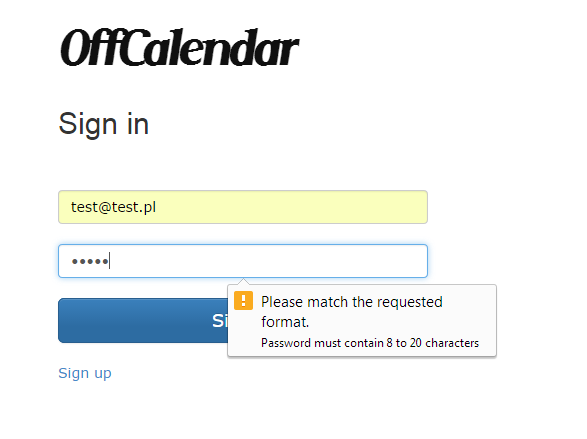
\includegraphics[width=0.5\textwidth]{signin.png}
\caption{Widok logowania użytkownika z przykładowym komunikatem ze standardu HTML5.}
\end{figure}

\begin{figure}[H]
\centering
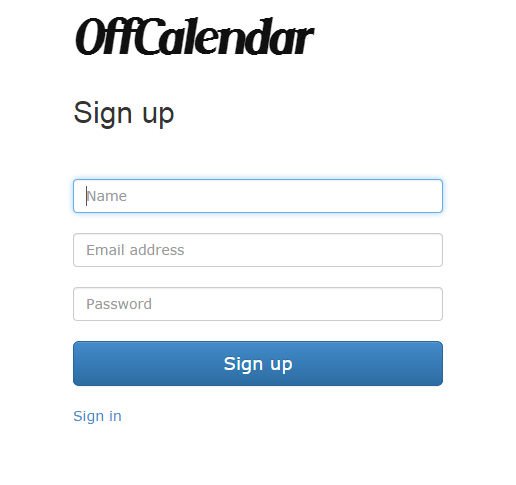
\includegraphics[width=0.5\textwidth]{register.png}
\caption{Widok rejestracji użytkownika.}
\end{figure}

Po pomyślnym utworzeniu konta i autoryzacji użytkownik zostaje przekierowany do głównego widoku aplikacji \textbf{dashboard}. Został on skonstruowany w taki sposób, aby załadować wszystkie potrzebne dane przy pierwszym wyświetleniu. Za pomocą atrybutu CSS \textbf{display: none} ukryto poszczególne sekcje. Przechodzenie pomiędzy nimi w menu polega na zmianie w/w atrybutu.

Główną część widoku zajmuje kalendarz wraz z przyciskami nawigacyjnymi. Utworzone wydarzenia możemy przeglądać na kilka określonych sposobów:

\begin{itemize}
\item w widoku rocznym z liczbą wydarzeń przypadających na dany miesiąc,
\item w widoku miesięcznym z graficzną reprezentacją wydarzeń z podziałem na dni miesiąca,
\item w widoku tygodniowym obrazującym harmonogram wraz z czasami trwania danych wydarzeń,
\item w widoku dziennym obrazującym wydarzenia wraz z godzinami rozpoczęcia oraz zakończenia.
\end{itemize}

W projekcie wykorzystano plugin \textbf{bootstrap-calendar}\footnote{\url{https://github.com/Serhioromano/bootstrap-calendar}}. Został on na potrzeby projektu rozszerzony o kompletny mechanizm dodawania, edycji oraz usuwania wydarzeń.

Oprócz przycisków nawigacyjnych, przenoszących pomiędzy widokami, w przestrzeni roboczej umieszczono przycisk \textbf{Add event} kierujący do widoku dziennego, gdzie istnieje możliwość dodawania nowych wydarzeń i edycji/usuwania istniejących. Poniższy zrzut ekranu obrazuje formularz dodawania nowego wydarzenia wraz z wcześniej utworzonym wydarzeniem w widoku dziennym.

\begin{figure}[H]
\centering
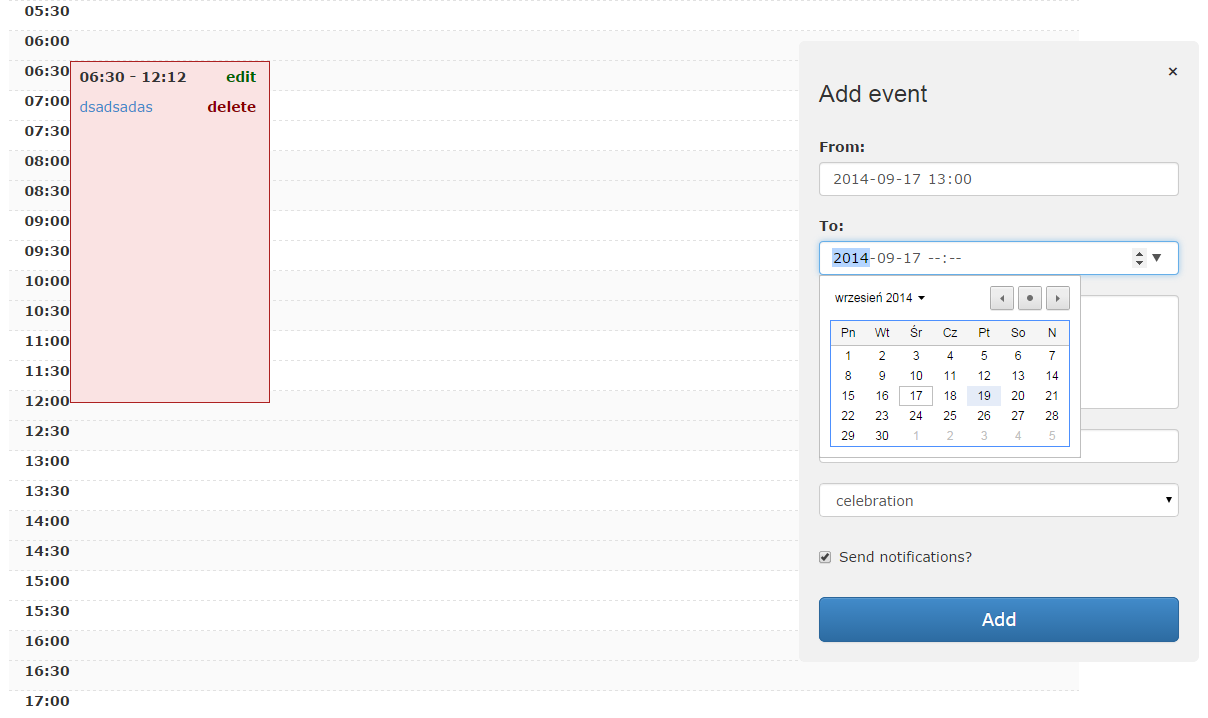
\includegraphics[width=0.9\textwidth]{add_event.png}
\caption{Formularz dodawania nowego wydarzenia w widoku dziennym.}
\end{figure}

Więcej nt. zarządzania wydarzeniami w sekcji 4.1.2.

Inicjacja kalendarza odbywa się w momencie załadowania widoku dashboard poprzez wywołanie metody \textbf{calendar}. Jako parametr przyjmuje ona opcje oraz kontekst. Opcje oznaczają parametry z jakimi wywołany zostanie kalendarz. Należą do nich m. in.

\begin{itemize}
\item szerokość kontenera,
\item widok początkowy (roczny, miesięczny, tygodniowy lub dzienny),
\item typ źródła danych (tablica, plik JSON, zewnętrzny plik),
\item ścieżka do katalogu zawierającego szablony widoków etc.
\end{itemize}

Kontekst definiowany jest przez element kodu HTML o określonym identyfikatorze (np. <div id=''kalendarz''></div>) w którym umieszczony zostanie kalendarz.

Widoki kalendarza ładowane są asynchroniczne. Zostały skonstruowane w HTML z zastosowaniem silnika szablonów JavaScript o nazwie \textbf{Underscore.js}\cite{underscore}. Separuje on warstwę danych od warstwy prezentacji i dostarcza wielu funkcji pozwalających operować na przekazanych do widoku zmiennych. Poniższy fragment uproszczonego kodu z widoku dziennego obrazuje prostą pętlę wyświetlającą wydarzenia.

\begin{lstlisting}[caption=Fragment kodu prezentujący składnię Underscore.js., label=amb, captionpos=b]

<% _.each(after_time, function(event){ %>
<div class="day-highlight dh-<%= event.class %>">
       		<span class="cal-hours"><%= event.start_hour %></span>
              	<%= event.description %></a>
       </div>
<% }); %>

\end{lstlisting}

Prócz głównego widoku kalendarza użytkownik ma możliwość przejścia do następujących sekcji:

\begin{itemize}
\item \textbf{Upcoming events:} lista wydarzeń nadchodzących,
\item \textbf{Ongoing events:} lista wydarzeń trwających,
\item \textbf{Past events:} lista wydarzeń zakończonych,
\item \textbf{Your profile:} dane użytkownika wraz z liczbą stworzonych wydarzeń oraz liczbą wydarzeń z aktywowanymi powiadomieniami.
\end{itemize}

Dodatkowo zaimplementowano uproszczony mechanizm wyszukiwania wydarzeń po treści. Kod funkcji \textbf{initSearch()} przedstawiono na poniższym listingu.

\begin{lstlisting}[caption=Wyszukiwanie wydarzeń w oparciu o treść., label=amb, captionpos=b]

OffCalendar.initSearch = function () {

    $(document).ready(function () {
    
        var $form = $('form[name=search_event]');

        $form.submit(function (event) {

            event.preventDefault();

            var userId = OffCalendar.user.id;
            var formData = $form.serializeArray();
            var searchTerm = formData[0]['value'];

            if (searchTerm !== '') {

                IndexedDB.searchEvent(userId, searchTerm, function (events) {

                    var $containers = $('.offcalendar-container');
                    var $searchContainer = $('#search-cont');

                    OffCalendar.appendEventsHTML($searchContainer, events);

                    $containers.hide();
                    $searchContainer.show();
                });
            }
        });
    });
};

\end{lstlisting}

Po zakończeniu pracy z aplikacją OffCalendar następuje wylogowanie (\textbf{Logout}), co w praktyce wiąże się z usunięciem zapisanych w obiekcie localStorage danych logowania.

\subsection{Zarządzanie wydarzeniami}
\label{sec:zarzWyd}

Ogół operacji związanych z manipulacją wydarzeniami (dodawanie, edycja oraz usuwanie) spoczywa na mechanizmie \textbf{IndexedDB}. Inicjacja obiektu bazy lokalnej następuje w momencie każdorazowego ładowania widoku dashboard. Poniższy kod obrazuje otwarcie połączenia z bazą danych.

\begin{lstlisting}[caption=Otwarcie połączenia z lokalną bazą danych., label=amb, captionpos=b]

IndexedDB.open = function (callback) {

    var request = indexedDB.open(DB_NAME, DB_VERSION);

    request.onupgradeneeded = function (e) {

        var db = e.target.result;

        e.target.transaction.onerror = IndexedDB.onerror;

        if (db.objectStoreNames.contains(DB_STORE_NAME)) {
            db.deleteObjectStore(DB_STORE_NAME);
        }

        var store = db.createObjectStore(DB_STORE_NAME, {keyPath: "remote_id", autoIncrement: true});

        store.createIndex('id', 'id', {unique: true});
        store.createIndex('user_id', 'user_id', {unique: false});
        store.createIndex('voided', 'voided', {unique: false});
        store.createIndex('remote_timestamp', 'remote_timestamp', {unique: false});
        store.createIndex('search', ['user_id', 'description'], {unique: false});

    };

    request.onsuccess = function (e) {
        IndexedDB.db = e.target.result;
        callback(true);
    };

    request.onerror = function (event) {
        callback(false);
    };
};

\end{lstlisting}

Baza lokalna zostaje otwarta z dwoma parametrami: nazwą bazy oraz jej wersją. Następnie tworzone są indeksy niezbędne do przeszukiwania po nazwach pól np. indeks o nazwie \textbf{search} wyszukuje pola \textbf{user\_id} oraz \textbf{description} i akceptuje duplikaty. Zarówno w przypadku pomyślnego jak i błędnego wykonania żądania wykonywana jest funkcja określona w parametrze callback. 

W aplikacji OffCalendar po otwarciu połączenia do bazy danych wykonywane jest pobranie wydarzeń dla danego użytkownika (kod poniżej) a następnie zainicjowanie synchronizacji

\begin{lstlisting}[caption=Pobranie wydarzeń użytkownika., label=amb, captionpos=b]

IndexedDB.getUserEvents = function (userId, callback) {

    var resultSet = [];

    var transaction = IndexedDB.db.transaction([DB_STORE_NAME], DB_TRANS_MODE_READ_ONLY);

    var store = transaction.objectStore(DB_STORE_NAME);

    var keyRange = IDBKeyRange.only(userId);

    var cursorRequest = store.index('user_id').openCursor(keyRange);

    cursorRequest.onsuccess = function (e) {

        var result = e.target.result;

        if (!!result === false)
            return;

        resultSet.push(result.value);

        result.continue();
    };

    transaction.oncomplete = function (event) {
        callback(resultSet);
    };

    cursorRequest.onerror = function (event) {
        callback(null);
    };
};

\end{lstlisting}

Flaga DB\_STORE\_NAME oznacza nazwę tabeli, natomiast DB\_TRANS\_MODE\_ONLY tryb dostępu (w tym przypadku wyłącznie odczyt). Następnie wykorzystywany jest indeks tworzony wraz z nową wersją bazy danych. Obiekt \textbf{cursorRequest} pozwala przeszukiwać tabelę i zapisywać rekordy (spełniające warunki określone w indeksie) do tablicy wynikowej \textbf{resultSet} wykorzystanej następnie w funkcji callback.

Pobrane wydarzenia zostają zapisane w opcjach kalendarza, po czym następuje jego renderowanie. Struktura obiektu reprezentującego przykładowe wydarzenie przedstawia się następująco:

\begin{lstlisting}[caption=Struktura obiektu reprezentującego wydarzenie., label=amb, captionpos=b]

class: "event-important"
start_timestamp: 1411349400000
end_timestamp: 1411380720000
last_update_timestamp: 0
remote_id: 1
remote_timestamp: 1411398325288
send_notification: 0
description: "test"
url: ""
user_id: 4
voided: 0

\end{lstlisting}

Poszczególne pola oznaczają kolejno: klasę wydarzenia (kolor), stempel czasowy rozpoczęcia wydarzenia, stempel czasowy zakończenia wydarzenia, stempel czasowy ostatniej synchronizacji (0 oznacza nowo dodane wydarzenie), identyfikator rekordu, stempel czasowy ostatniej aktualizacji wydarzenia przez użytkownika, flagę informującą o wysyłaniu powiadomień \mbox{e-mail}, opis wydarzenia, zewnętrzny adres url, id użytkownika oraz flagę informującą o usunięciu danego wydarzenia (ustawiona na wartość 1 oznacza, że użytkownik usunął wydarzenie).

Dodawanie, edycja oraz usuwanie wydarzeń odbywa się widoku dziennym. Przedstawia on godziny dnia w odstępie 30 minutowym. Kliknięcie na każdą z nich otwiera okno dodawania nowego wydarzenia z odpowiednio uzupełnioną datą rozpoczęcia. W przypadku edycji wydarzenia to samo okno zostaje uzupełnione również o wszystkie pozostałe dane wydarzenia. Poniższy kod obrazuje operację edycji.

\begin{lstlisting}[caption=Edycja wydarzenia cz. 1., label=amb, captionpos=b]

IndexedDB.updateEvent = function (eventRemoteId, eventPropertiesToUpdate, callback) {

    var trans = IndexedDB.db.transaction([DB_STORE_NAME], DB_TRANS_MODE_READ_WRITE);

    var store = trans.objectStore(DB_STORE_NAME);

    var cursorRequest = store.openCursor(IDBKeyRange.only(eventRemoteId));

    cursorRequest.onsuccess = function (e) {

        var cursor = cursorRequest.result || e.result;

        var Event = cursor.value;

        for (var property in eventPropertiesToUpdate) {
            Event[property] = eventPropertiesToUpdate[property];
        }

        var request = cursor.update(Event);

        request.onerror = function (e) {
            callback(null);
        };

        request.onsuccess = function (e) {
            callback(Event);
        };
    };
};

\end{lstlisting}

W przypadku poprawnego dodania wydarzenia wykonywana jest funkcja callback. W aplikacji \mbox{OffCalendar} użytkownik zostanie poinformowany o efekcie żądania i przekierowany na stronę główną. Następny listing obrazuje operację pobrania danych z formularza edycji wydarzenia i przekazania ich do powyższej funkcji oraz przekierowanie realizowane z użyciem odpowiedniej funkcji zwrotnej.

\begin{lstlisting}[caption=Edycja wydarzenia cz. 2., label=amb, captionpos=b]

OffCalendar.initEventUpdate = function () {

    var $form = $('form[name=offcalendar_update_event]');

    $form.submit(function (event) {

        event.preventDefault();

        var formData = $form.serializeArray();

        var userId = OffCalendar.user.id;

        var startTimestamp = OffCalendarHelper.getTimestampFromDate(formData[0]['value']);
        var endTimestamp = OffCalendarHelper.getTimestampFromDate(formData[1]['value']);

        var description = formData[2]['value'];

        var url = formData[3]['value'];
        var eventClass = OffCalendarHelper.mapEventTypeToClassName(formData[4]['value']);

        var sendNotification = $('input#send_notification').is(':checked');

        var toUpdate = {
            user_id: userId,
            start_timestamp: startTimestamp,
            end_timestamp: endTimestamp,
            description: description,
            url: url,
            class: eventClass,
            send_notification: sendNotification ? 1 : 0,
            voided: 0,
            remote_timestamp: OffCalendarHelper.currentTimestamp()
        };

        var eventRemoteId = formData[5]['value'];
        eventRemoteId = parseInt(eventRemoteId, 10);

        IndexedDB.updateEvent(eventRemoteId, toUpdate, function (Event) {
            if (Event !== null) {
                OffCalendar.showFlashMessage('success', 'Event succesfully updated!', function () {
                    window.location = OffCalendar.dashboardUrl;
                });
            }
        });
    });

};

\end{lstlisting}

Dodawanie wydarzenia wykonywane jest analogicznie. Z kolei operacja usuwania polega na zmianie atrybutu \textbf{voided} na wartość 1. Jest to konieczne z uwagi na synchronizację wydarzeń pomiędzy różnymi urządzeniami: całkowite usunięcie konkretnego obiektu z bazy lokalnej mogłoby prowadzić do konfliktów.

Pozostałe operacje związane z manipulacją wydarzeniami sprowadzają się do pobrania tablicy obiektów \textbf{Event}, analizy pod względem daty rozpoczęcia i zakończenia oraz klasyfikacji poprzez umieszczenie w jednej z sekcji dostępnych w menu (Past Events, Ongoing Events, Upcoming Events).

Zarówno dodawanie, usuwanie jak i edycja wydarzenia kończy się przekierowaniem do głównej strony aplikacji i wywołaniem synchronizacji z częścią serwerową poprzedzoną weryfikacją obecności połączenia internetowego.

\subsection{Detekcja połączenia internetowego}
\label{sec:detPolInt}

W związku z faktem, że aplikacja OffCalendar oferuje również wsparcie dla trybu online, automatyczna detekcja stanu połączenia internetowego jest kluczowa. Posiadanie dostępu do sieci Internet umożliwia autoryzację oraz, co najważniejsze, synchronizację danych lokalnych z główną bazą będącą częścią części serwerowej projektu.

W aplikacji zastosowano bibliotekę Offline.js \footnote{\url{http://github.hubspot.com/offline/docs/welcome/}}. Oferuje ona automatyczną detekcję połączenia wraz z powiadomieniami o jego stanie oraz możliwość wykonania próby jego ponowienia. Wraz z logiką biblioteki twórcy zaproponowali szablony komunikatów podlegające pełnej personalizacji.

Działanie biblioteki opiera się na cyklicznym wykonywaniu żądania AJAX pobrania niewielkiego zasobu graficznego (1x1 pikseli) w formacie png o rozmiarze 110 bajtów. Wybór ten umożliwia odwołanie do zasobu znajdującego się pod innym adresem, ponieważ koncepcja \textbf{Same-origin policy}\footnote{Same-origin policy, inaczej zasada tożsamego pochodzenia, zezwala na dostęp do zasobów stron, których adres wyróżnia się takim samym protokołem, nazwą domeny serwera i numerem portu\cite{sameOrigin}} nie odnosi się do obiektów graficznych.

Inicjacja biblioteki wykonywana jest w momencie załadowania widoku głównego. Polega ona na podaniu kilku opcji przedstawionych na poniższym listingu.

\begin{lstlisting}[caption=Inicjalizacja biblioteki Offline.js badającej stan połączenia internetowego., label=amb, captionpos=b]

Offline.options = {
	checks: {
   	   image: {
            url: '[adres_url]/blank.png?_=' + (Math.floor(Math.random() * 1000000000))
       },
       active: 'image'
    },
    reconnect: false,
    checkOnLoad: true
};

\end{lstlisting}

\begin{itemize}
\item \textbf{url:} oznacza adres zasobu graficznego; dodany kod oblicza pseudo-losowy numer i dokleja go do adresu url żądania, celem uniknięcia cache-owania wskazanego pliku png,
\item \textbf{active:} oznacza typ zasobu - biblioteka oferuje bowiem również sprawdzanie stanu połączenia w oparciu o skrypt,
\item \textbf{reconnect:} flaga informująca o konieczności ponawiania połączenia - w projekcie zbędna z uwagi na fakt, że dysponowanie aktywnym połączeniem sieciowym nie jest konieczne do prawidłowego funkcjonowania aplikacji,
\item \textbf{checkOnLoad:} flaga informująca o konieczności wykonania testu połączenia w momencie załadowania widoku głównego.
\end{itemize}

Żądanie opiera się na właściwościach obiektu \textbf{XMLHttpRequest} zapewniających asynchroniczne wykonanie, czyli bez przeładowania strony. Poniżej kod głównej metody checkXHR(xhr, onUp, onDown) sprawdzającej stan połączenia internetowego w oparciu o opcje obiektu XMLHttpRequest (xhr) ustawione w momencie inicjalizacji biblioteki i wywołującego funkcje callback.

\begin{lstlisting}[caption=Metoda checkXHR() wykonująca żądanie AJAX załadowania zasobu graficznego., label=amb, captionpos=b]
checkXHR = function(xhr, onUp, onDown) {
        var checkStatus, _onerror, _onload, _onreadystatechange, _ontimeout;
        checkStatus = function() {
            if (xhr.status && xhr.status < 12000) {
                return onUp();
            } else {
                return onDown();
            }
        };
        if (xhr.onprogress === null) {
            _onerror = xhr.onerror;
            xhr.onerror = function() {
                onDown();
                return typeof _onerror === "function" ? _onerror.apply(null, arguments) : void 0;
            };
            _ontimeout = xhr.ontimeout;
            xhr.ontimeout = function() {
                onDown();
                return typeof _ontimeout === "function" ? _ontimeout.apply(null, arguments) : void 0;
            };
            _onload = xhr.onload;
            return xhr.onload = function() {
                checkStatus();
                return typeof _onload === "function" ? _onload.apply(null, arguments) : void 0;
            };
        } else {
            _onreadystatechange = xhr.onreadystatechange;
            return xhr.onreadystatechange = function() {
                if (xhr.readyState === 4) {
                    checkStatus();
                } else if (xhr.readyState === 0) {
                    onDown();
                }
                return typeof _onreadystatechange === "function" ? _onreadystatechange.apply(null, arguments) : void 0;
            };
        }};
\end{lstlisting}

Tylko w sytuacji, w której połączenie internetowe jest aktywne wykonywana jest synchronizacja wydarzeń. Poniżej wygląd komunikatów informujących o pracy w trybie online/offline.

\begin{figure}[H]
\centering

\includegraphics[width=0.9\textwidth]{isOnline.png}
\caption{Komunikat o przejściu w tryb online.}
\end{figure}

\begin{figure}[H]
\centering

\includegraphics[width=0.9\textwidth]{isOffline.png}
\caption{Komunikat o przejściu w tryb offline.}
\end{figure}

\subsection{Synchronizacja danych}
\label{autSynDanych}

Proces synchronizacji danych jest uruchamiany co 3 minuty, a także po dodaniu, edycji lub usunięciu wydarzenia. Proces rozpoczyna się w momencie wywołania metody synchronize. Do funkcji przekazane są dane użytkownika, adres URL interfejsu programowania odpowiedzialnego za proces po stronie serwerowej aplikacji oraz funkcja, która zostanie wywołana po zakończeniu synchronizacji.

\begin{lstlisting}[caption=Funkcja synchronize rozpoczynająca proces synchronizacji., label=amb, captionpos=b]
IndexedDB.synchronize = function(userId, userEmail, userPassword, eventsSyncApiUrl, callback) {

	if (IndexedDB.sync.inProgress === true) {
    	return;
	}

	IndexedDB.sync.inProgress = true;
	IndexedDB.sync.userId = userId;
	IndexedDB.sync.remoteTimestamp = OffCalendarHelper.currentTimestamp();
	IndexedDB.sync.itemsSynced = 0;
	IndexedDB.sync.email = userEmail;
	IndexedDB.sync.password = userPassword;
	IndexedDB.sync.url = eventsSyncApiUrl;
	IndexedDB.sync.callback = callback;

	var lastRemoteSyncTimestamp = IndexedDB.sync.getLastRemoteSyncTimestamp(userId);

	IndexedDB.getUserEventsForSync(userId, lastRemoteSyncTimestamp, IndexedDB.sync.eventsFetched);


};
\end{lstlisting}

W przypadku gdy proces synchronizacji jest w trakcie wykonania (atrybut  IndexedDB.sync.inProgress posiada wartość true) kolejne wywołania metody będą odwoływane aż do chwili zakończenia procesu synchronizacji. Metoda ta pobiera stempel czasowy ostatniej synchronizacji oraz wydarzenia które zostały zmodyfikowane od czasu ostatniej synchronizacji.

Po pomyślnym pobraniu wydarzeń tworzone jest zapytanie AJAX wysyłające je do części serwerowej w celu ich synchronizacji.

\begin{lstlisting}[caption=Wysłanie żądania synchronizacji do części serwerowej., label=amb, captionpos=b]

IndexedDB.sync.eventsFetched = function(events) {

	if (events === null) {
    	IndexedDB.sync.failed('Error fetching events from db.');
	}

	var lastSyncTimestamp = IndexedDB.sync.getLastSyncTimestamp();

	var request = $.ajax({
    	url: IndexedDB.sync.url,
    	dataType: "json",
    	type: "POST",
    	data: {
        	email: IndexedDB.sync.email,
        	password: IndexedDB.sync.password,
        	last_sync_timestamp: lastSyncTimestamp,
        	events: JSON.stringify(events)
    	}
	});

	request.done(function(response, textStatus, jqXHR) {

    	IndexedDB.sync.processData(response);

	});

	request.fail(function(jqXHR, textStatus, errorThrown) {

    	var msg;

    	if (jqXHR.responseJSON && jqXHR.responseJSON.error) {
        	msg = jqXHR.responseJSON.error;
    	} else {
        	msg = jqXHR.status + ' - ' + errorThrown;
    	}

    	IndexedDB.sync.failed(msg);

	});

};
\end{lstlisting}

Część serwerowa zwraca zsynchronizowaną listę wydarzeń. Wydarzenia te zostają zaktualizowane w lokalnej bazie danych. Poniżej przedstawiona jest funkcja dokonująca aktualizacji.

\begin{lstlisting}[caption=Aktualizacja wydarzeń przechowywanych w lokalnej bazie danych., label=amb, captionpos=b]

IndexedDB.sync.updateEvents = function() {

	if (IndexedDB.sync.eventsToUpdate.length > 0) {

    	var Event = IndexedDB.sync.eventsToUpdate.pop();

    	if (Event.id) {
        	IndexedDB.updateEventById(Event.id, Event, IndexedDB.sync.updateEvents);
    	} else {
        	IndexedDB.updateEvent(Event.remote_id, Event, IndexedDB.sync.updateEvents);
    	}

    	IndexedDB.sync.itemsSynced++;

	} else {

    	IndexedDB.sync.success();

	}

};

\end{lstlisting}

Po zakończeniu aktualizacji proces synchronizacji dobiega końca. Przed zakończeniem konieczne jest zaktualizowanie stempli czasowych - zarówno wygenerowanego po stronie klienta jak i serwera.

\begin{lstlisting}[caption=Kod finalizujący proces synchronizacji., label=amb, captionpos=b]

IndexedDB.sync.success = function() {

	IndexedDB.sync.inProgress = false;

	IndexedDB.sync.setLastRemoteSyncTimestamp(IndexedDB.sync.remoteTimestamp);
    
	IndexedDB.sync.setLastSyncTimestamp(IndexedDB.sync.timestamp);

	IndexedDB.sync.callback(IndexedDB.sync.itemsSynced);

};

\end{lstlisting}

Po wykonaniu aktualizacji stempli oraz zaktualizowaniu flagi wskazującej na to, że proces synchronizacji jest w toku wywoływana jest, przekazana na początku procesu, funkcja. Jej argumentem jest ilość wydarzeń które zostały zsynchronizowane.

\section{Aplikacja serwerowa}
\label{sec:apSerw}

Aby aplikacja OffCalendar działała prawidłowo, konieczna była implementacja mechanizmów dostępu do bazy danych i zarządzania danymi oraz implementacja bezstanowych interfejsów odpowiadających za komunikację z częścią kliencką aplikacji.

Największym problemem, który należało rozwiązać, były różnice w strukturze obiektów przechowywanych po stronie klienckiej oraz serwerowej. Mechanizmy odpowiedzialne za zarządzanie wydarzeniami musiały zostać zaimplementowane w taki sposób, aby umożliwiały łatwą konwersję oraz porównywanie różnych typów wydarzeń.

\subsection{Implementacja warstwy danych}
\label{komBazaDanych}

Pierwszym z elementów, który musiał zostać wykonany w części serwerowej aplikacji była warstwa danych. Składają się na nią: 

\begin{enumerate}
\item klasy wykonujące operacje CRUD oparte na klasie ActiveRecord\cite{ciActiveRecord} frameworku CodeIgniter:
\begin{itemize}
\item \textbf{Events\_model}
\item \textbf{Users\_model}
\end{itemize}
\item klasy służące do mapowania rekordów przechowywanych w bazach danych (klienckiej oraz serwerowej) na poszczególne obiekty:
\begin{itemize}
\item \textbf{Event}
\item \textbf{User}
\end{itemize}
\end{enumerate}

Wydarzenia (Event) są tworzone po stronie aplikacji klienckiej i każdemu z nich jest przypisywana unikalna wartość lokalnego klucza głównego. Dodatkowo każde wydarzenie przechowywane w bazie danych posiada również klucz główny generowany przez bazę danych. Z tego względu, przy inicjalizacji oraz zapisie do bazy danych obiektów wydarzeń, powyższe różnice musiały zostać odpowiednio obsłużone.

Dobrym przykładem jest kod konstruktora klasy Event, który sprawdza obecność obydwu kluczy głównych i na ich podstawie odpowiednio inicjuje obiekt.

\definecolor{dkgreen}{rgb}{0,.6,0}

\lstset{
  language        = php,
  basicstyle      = \small\ttfamily,
  keywordstyle    = \color{blue},
  stringstyle     = \color{orange},
  identifierstyle = \color{dkgreen},
  commentstyle    = \color{gray},
  emph            =[1]{php},
  emphstyle       =[1]\color{black},
  emph            =[2]{__construct,int,string,public,private,function,try,throw,catch,\$this,return,if,and,or,else,foreach},
  emphstyle       =[2]\color{blue},
  showstringspaces=false
}

\begin{lstlisting}[caption=Fragment konstruktora klasy Event., label=amb, captionpos=b]

public function __construct($properties = array()) {
    if ($properties) {
        if (isset($properties['id']) && $properties['id']) {
            $this->id = (int) $properties['id'];
        }

        if (isset($properties['remote_id']) && $properties['remote_id']) {
            $this->remoteId = (int) $properties['remote_id'];
        }

        $this->userId = (int) $properties['user_id'];
        $this->startTimestamp = (int) $properties['start_timestamp'];
        $this->endTimestamp = (int) $properties['end_timestamp'];
        $this->description = (string) $properties['description'];
        $this->sendNotification = (int) $properties['send_notification'];
        $this->voided = (int) $properties['voided'];
        $this->remoteTimestamp = (int) $properties['remote_timestamp'];
        $this->lastUpdateTimestamp = (int) $properties['last_update_timestamp'];
    }
}

\end{lstlisting}

W zależności czy dane wydarzenie ma zostać zapisane w bazie danych czy też zwrócone do aplikacji klienckiej, musi ono zawierać odpowiedni zestaw atrybutów. Do tego celu stworzone zostały poniższe metody klasy Event.

\begin{lstlisting}[caption=Serializacja obiektu Event., label=amb, captionpos=b]

public function toDbArray() {
    return array(
        'user_id' => $this->userId,
        'start_timestamp' => $this->startTimestamp,
        'end_timestamp' => $this->endTimestamp,
        'description' => $this->description,
        'send_notification' => $this->sendNotification,
        'voided' => $this->voided,
        'remote_timestamp' => $this->remoteTimestamp,
        'last_update_timestamp' => $this->lastUpdateTimestamp,
    );
}

public function toApiArray() {
    $arr = $this->toDbArray();

    $additional = array(
    	'id' => $this->id,
    );

    if ($this->remoteId) {
    	$additional['remote_id'] = $this->remoteId;
    }

    return array_merge($additional, $arr);
}

\end{lstlisting}

Dla wydarzeń posiadających klucz główny wygenerowany w bazie danych, aktualizacja dokonywana jest na jego podstawie. W przeciwnym wypadku dla danego wydarzenia utworzony zostaje nowy rekord w bazie danych.

\begin{lstlisting}[caption=Aktualizacja obiektu Event w bazie danych., label=amb, captionpos=b]

function persist() {
   	if ($this->id) {
       		$this->_ci->events_model->updateEvent($this->id, $this->toDbArray());
   	} else {
       		$this->id = $this->_ci->events_model->addEvent($this->toDbArray());
   	}

   	return $this;
}

\end{lstlisting}

Klasa Events\_model bezpośrednio odpowiada za manipulację rekordami znajdującymi się w bazie danych. Bogaty zbiór metod klasy ActiveRecord pozwala na łatwe wykonanie operacji tworzenia, pobierania oraz aktualizacji rekordów.

\begin{lstlisting}[caption=Przykładowe metody klasy Events\_model odpowiedzialne za komunikację z bazą danych., label=amb, captionpos=b]

function getEventById($eventId) {
	
   $query = $this->db->get_where('events', array('id' => $eventId));

   return $query->row_array();
}

function updateEvent($eventId, $toUpdate) {

   $this->db->update('events', $toUpdate, array('id' => $eventId));

   return $this->db->affected_rows();
}

function addEvent($event) {
   	
   $this->db->insert('events', $event);

   return $this->db->insert_id();
}

\end{lstlisting}

Klasy User oraz Users\_model zostały stworzone analogicznie do klas Events oraz Events\_model. Różnicą jest tutaj brak klucza głównego generowanego po stronie klienta. Wynika to z faktu, iż konta użytkowników mogą być tworzone wyłącznie w trybie online. Pozwala to na uniknięcie narzutu spowodowanego koniecznością przechowywania podwójnych kluczy głównych.

\subsection{Bezstanowe interfejsy}
\label{bezstInter}

W celu komunikacji z częścią kliencką stworzone zostały interfejsy programowania aplikacji umożliwiające manipulację danymi użytkowników oraz synchronizację wydarzeń. Ze względu na nacisk położony na tryb offline interfejsy zostały stworzone zgodnie z zasadami architektury REST. W celu minimalizacji danych przesyłanych do klienta, odpowiedzi zawierają dane w formacie JSON.

Większość metod używanych przez interfejsy wymaga wcześniejszej autentykacji użytkownika. Wyjątkiem jest tutaj metoda register interfejsu Users\_api pozwalająca na rejestrację nowych użytkowników.

\begin{lstlisting}[caption=Rejestracja użytkowników przy użyciu metody register interfejsu Users\_api., label=amb, captionpos=b]

function register() {
  try {
      if (!$this->input->post()) {
      	throw new Exception('Please fill required fields');
      }

      $fields = $this->users->getFieldsValidationRules(array('name', 'email', 'password'));

      $this->form_validation->set_rules($fields);

      if (!$this->form_validation->run()) {
      	throw new Exception(strip_tags(validation_errors()));
      }

      $vals = array();

      foreach (array_keys($fields) as $f) {
      	$vals[] = $this->form_validation->set_value($f);
      }

      list($name, $email, $password) = $vals;

      $user = $this->users->register($name, $email, $password);

      return $this->jsonResponse($user->toApiResponse());
  } catch (Exception $e) {
      return $this->jsonError($e->getMessage());
  }
}

\end{lstlisting}

Metoda register w pierwszej kolejności sprawdza poprawność danych przesłanych przez aplikację kliencką. W przypadku błędu do aplikacji klienckiej zwracana jest odpowiednia wiadomość oraz kod błędu. Po pomyślnym utworzeniu nowego konta, odpowiedź zawiera  dane użytkownika, w których znajduje się m. in. jego unikalny identyfikator, na podstawie którego można zidentyfikować przechowywane w lokalnej bazie danych rekordy do niego należące.

Wspólną dla wszystkich interfejsów programowania jest funkcja odpowiadająca za autentykację użytkownika. Ze względu na bezstanowość, przy każdym żądaniu synchronizacji danych czy aktualizacji danych użytkownika, konieczne jest potwierdzenie jego tożsamości.

\begin{lstlisting}[caption=Rejestracja użytkowników przy użyciu metody register interfejsu Users\_api., label=amb, captionpos=b]

private function authenticateUser() {
  try {
	$email = (string) $this->input->post('email');

	$password = (string) $this->input->post('password');

	$user = $this->users->login($email, $password);

    return $user;
  } catch (Exception $e) {
	throw new Exception('Authentication failed.');
  }
}

\end{lstlisting}

Powyższa metoda w przypadku pomyślnej autentykacji zwraca obiekt User, natomiast w przypadku niezgodności przesłanych danych rzucany jest odpowiedni wyjątek informujący, że proces autentykacji się nie powiódł.

\subsection{Synchronizacja danych}
\label{serwSynDanych}

Najbardziej złożonym procesem wykonywanym w aplikacji OffCalendar jest synchronizacja danych. Część serwerowa tego procesu rozpoczyna się w momencie przesłania przez część kliencką żądania synchronizacji. Żądanie musi zawierać dane wymagane do autentykacji użytkownika, stempel czasowy określający czas ostatniej synchronizacji oraz listę wydarzeń, które uległy modyfikacji od czasu ostatniej synchronizacji.

\begin{lstlisting}[caption=Metoda synchronize interfejsu programowania Events\_api., label=amb, captionpos=b]
function synchronize() {
   	try {
	   $user = $this->authenticateUser();

       $userId = $user->getId();

       $lastSyncTimestamp = (int)$this->input->post('last_sync_timestamp');
       $currTimestamp = time();

       $dbEvents = $this->events->getDbEventsForSynchronization($userId, $lastSyncTimestamp);       	 
       $postEvents = $this->input->post('events');

       $remoteEvents = $this->events->getEventsFromPostData($postEvents, $user);
      	 
       $eventsToUpdate = $this->events->synchronize($remoteEvents, $dbEvents, $currTimestamp);

       $toUpdate = array();
       	 
       foreach($eventsToUpdate as $e){
          $toUpdate[] = $e->toApiArray();
       }

       $response = array(
          'sync_timestamp' => $currTimestamp,
          'events_to_update' => $toUpdate,
       );

       return $this->jsonResponse($response);
    } catch (Exception $e) {

      return $this->jsonError($e->getMessage());
  }
}

\end{lstlisting}

Powyższa metoda sprawdza poprawność przesłanych przez część kliencką danych oraz przekazuje komponentowi Events dane potrzebne do poprawnej modyfikacji wydarzeń. Komponent Events zwraca listę zaktualizowanych wydarzeń, które zostaną przesłane do części klienckiej celem aktualizacji wydarzeń w lokalnej bazie danych. Do odpowiedzi zostaje dołączony również stempel czasowy synchronizacji.

\begin{lstlisting}[caption=Modyfikacja wydarzeń w metodzie synchronize komponentu Events., label=amb, captionpos=b]

public function synchronize($remoteEvents, $dbEvents, $currTimestamp) {
   	$toUpdate = array();

   	foreach ($remoteEvents as $remoteEvent) {

      if (!$remoteEvent->hasId()) {

	      $remoteEvent->setLastUpdateTimestamp($currTimestamp);

          $remoteEvent->persist();

          $toUpdate[] = $remoteEvent;

          continue;
      }

      $eventId = $remoteEvent->getId();

      if (isset($dbEvents[$eventId])) {

          $dbEvent = $dbEvents[$eventId];

          if ($dbEvent->getRemoteTimestamp() > $remoteEvent->getRemoteTimestamp()) {
          	$dbEvent->setRemoteId($remoteEvent->getRemoteId());
            $toUpdate[] = $dbEvent;
          } else {
            $remoteEvent->setLastUpdateTimestamp($currTimestamp);
            $remoteEvent->persist();
            $toUpdate[] = $remoteEvent;
          }

          unset($dbEvents[$eventId]);
      }
    }

    foreach ($dbEvents as $dbEvent) {

       	$toUpdate[] = $dbEvent;
    }

   	return $toUpdate;
}

\end{lstlisting}

Metoda synchronize komponentu events dzieli wydarzenia na wyszczególnione na etapie projektu (3.3.3) kategorie. Wydarzenia przesłane przez część kliencką zawierają wartość klucza głównego wygenerowanego przez lokalną bazę danych co umożliwia wydajną aktualizację rekordów. W przypadku wydarzeń, które zostały zmodyfikowane na innym urządzeniu obecny jest jedynie klucz główny wygenerowany na serwerze. Na jego podstawie aplikacja kliencka musi zadecydować o stworzeniu nowego rekordu lub aktualizacji już istniejącego.

\chapter{Instrukcja użytkownika}
\label{cha:instrUzytk}

W rozdziale tym szczegółowo opisany został sposób instalacji oraz konfiguracji aplikacji OffCalendar. Ponadto rozdział zawiera kompletną instrukcję obsługi aplikacji obejmującą zarządzanie kontami oraz wydarzeniami użytkownika.

\section{Instalacja i konfiguracja}
\label{sec:instKonf}

Do poprawnego działania aplikacji OffCalendar wymagane jest posiadanie następujących komponentów:

\begin{itemize}
\item Apache HTTP Server w wersji 2.2 lub nowszej
\item PHP x64 w wersji 5.5 lub nowszej
\item MySQL w wersji 5.6 lub nowszej
\end{itemize}

Najprostszą formą zainstalowania trzech powyższych komponentów jest skorzystanie z gotowych paczek oprogramowania zawierających zarówno serwer Apache jak i PHP oraz MySQL. W przypadku systemu Windows jedną z takich paczek jest to XAMPP, natomiast dla systemu Unix jest to Tasksel.

Po pomyślnej instalacji wszystkich komponentów konieczna jest odpowiednia konfiguracja aplikacji. Pierwszym z kroków jest dodatkowy wpis VirtualHost dla serwera Apache. Dla systemu Windows oraz domyślnej instalacji ścieżka do pliku konfiguracyjnego to \url{C:\xampp\apache\conf\extra\httpd-vhosts.conf}. Dla systemów Unix jest to \url{/etc/httpd/conf/httpd.conf}.

\begin{lstlisting}[caption=Konfiguracja serwera Apache., label=amb, captionpos=b]

<VirtualHost *:80>
    ServerAdmin webmaster@localhost
    DocumentRoot __PATH__
    ServerName __HOST__

    <Directory "__PATH__">
   	 AllowOverride All
   	 Order allow,deny
   	 Allow from all
            	Require all granted
    </Directory>
</VirtualHost>

\end{lstlisting}

Zmienna \_\_PATH\_\_ powinna zostać zastąpiona przez ścieżkę do projektu OffCalendar znajdującego się w \url{/projekt magisterski/offcalendar/}. Zmienna \_\_HOST\_\_ powinna zostać zastąpiona przez nazwę domeny która będzie używana do dostępu do aplikacji. W przypadku chęci skorzystania z domyślnej domeny zmienna powinna przyjąć wartość localhost.

Projekt OffCalendar musi posiadać wiedzę o domenie pod którą jest dostępny. W tym celu należy dokonać edycji pliku \url{/projekt magisterski/offcalendar/application/config/config.php}. Wymagana jest edycja zmiennej \_\_URL\_\_ na adres URL pod którym dostępna będzie aplikacja OffCalendar. Przy korzystaniu z domyślnej domeny zmienna \_\_URL\_\_ powinna mieć wartość \url{http://localhost/}.

\begin{lstlisting}[caption=Konfiguracja adresu URL dla projektu OffCalendar., label=amb, captionpos=b]

$config['base_url'] = '__URL__';

\end{lstlisting}

Kolejnym krokiem jest konfiguracja bazy danych. Po utworzeniu nowej bazy danych na serwerze MySQL konieczne jest wykonanie kwerend tworzących w niej odpowiednie struktury. Kwerendy znajdują się w pliku \url{/projekt magisterski/komponenty/mysql/offcalendar.sql}.

Do poprawnego połączenia z bazą danych konieczna jest edycja danych znajdujących się w \url{/projekt magisterski/offcalendar/application/config/database.php}. Pola wymagające edycji to \_\_HOST\_\_, \_\_USER\_\_, \_\_PASSWORD\_\_ oraz \_\_DATABASE\_\_.

\begin{lstlisting}[caption=Konfiguracja dostępu do bazy danych., label=amb, captionpos=b]

$db['default']['hostname'] = '__HOST__';
$db['default']['username'] = '__USER__';
$db['default']['password'] = '__PASSWORD__';
$db['default']['database'] = '__DATABASE__';

\end{lstlisting}

Po wykonaniu powyższych kroków aplikacja powinna być dostępna z poziomu przeglądarki internetowej (adres strony zgodny ze zmienną \_\_URL\_\_).

\section{Obsługa aplikacji}
\label{sec:obslAp}

Ogół akcji realizowanych w ramach aplikacji odbywa się wyłącznie za pomocą przeglądarki internetowej. Prosty i przejrzysty interfejs ułatwia korzystanie z pogramu, a ograniczona liczba widoku przyśpiesza wykonywanie podstawowych zadań.

\subsection{Zarządzanie wydarzeniami}
\label{sec:instrZarzWyd}

Wszystkie czynności wykonywane są w widoku przestrzeni roboczej (\url{__URL__/welcome/dashboard}) który dostępny jest po poprawnej autoryzacji. Podstawową funkcjonalnością aplikacji OffCalendar jest oczywiście zarządzanie wydarzeniami. Obejmuje ono:

\begin{itemize}
\item dodawanie nowych wydarzeń,
\item edycję wydarzeń istniejących,
\item usuwanie wydarzeń,
\item przeszukiwanie wydarzeń,
\item przeglądanie wydarzeń.
\end{itemize}

\textbf{Dodawanie} odbywa się poprzez przejście do widoku dziennego (przycisk "Add event" lub "Day"). Formularz wyświetlany jest po kliknięciu w belkę reprezentującą godzinę dnia (odstęp 30 minut). Po prawej stronie widoku przestrzeni roboczej pojawia się okno wraz z polami tekstowymi. Oznaczają one kolejno: godzinę rozpoczęcia wydarzenia (domyślnie wypełniona), godzinę zakończenia wydarzenia, opis wydarzenia, zewnętrzny adres url (opcjonalne), typ wydarzenia (do wyboru: regular, important, celebration, warning, party) oraz flaga dotycząca wysyłania notyfikacji e-mail. Po poprawnym dodaniu wydarzenia użytkownik zostaje przekierowany na stronę główną do widoku miesięcznego, który w postaci graficznej reprezentuje dodane wydarzenia.

\textbf{Edycja} przedstawia się analogicznie do dodawania; jedyną różnicę stanowi fakt, iż w momencie przejścia do odpowiedniego formularza wszystkie pola są wypełnione wartościami zapisanymi uprzednio w pamięci lokalnej przeglądarki. Formularz edycji wyświetlany jest po kliknięciu w przycisk "edit" znajdujący się w prawym górnym rogu wydarzenia w widoku dziennym.

\textbf{Usuwanie} realizowane jest poprzez kliknięcie przycisku "delete" w widoku dziennym dla danego wydarzenia.

\textbf{Przeszukiwanie} wywoływane jest w dowolnym widoku po podaniu szukanej frazy i zatwierdzeniu przyciskiem lupy. Z uwagi na ograniczenia mechanizmu IndexedDB efektywne wyszukiwanie odbywa się po podaniu pierwszych wyrazów (lub ich części) opisu wydarzenia.

\textbf{Przeglądanie} możliwe jest z wykorzystaniem kilku widoków:

\begin{itemize}
\item rocznego z liczbą wydarzeń przypadających na dany miesiąc,
\item miesięcznego (widok domyślny) z graficznym oznaczeniem wydarzeń w poszczególnych dniach miesiąca,
\item tygodniowego z podziałem na wydarzenia przypadające na poszczególne dni tygodnia,
\item dziennego z podziałem na godziny dnia.
\end{itemize}

Ponadto użytkownik ma możliwość przejrzenia wydarzeń z przeszłości, obecnie trwających oraz nadchodzących wybierając odpowiednią sekcję z menu po lewej stronie obszaru przestrzeni roboczej. W sekcji \textbf{Your Profile} znajdzie także informacje na temat liczby dodanych wydarzeń oraz otrzymywanych notyfikacji obok informacji dotyczących danych logowania.

\subsection{Zarządzanie kontami}
\label{sec:zarzKont}

Widokiem startowym aplikacji OffCalendar jest widok logowania. Aby dokonać pomyślnej autoryzacji należy założyć konto użytkownika. W tym celu wystarczy przejść do sekcji \textbf{Sign up}, która zawiera ekran rejestracji.

Aby utworzyć konto w serwisie wystarczy podać nazwę użytkownika, adres e-mail (niezbędny do przesyłania notyfikacji dotyczących wydarzeń) oraz hasło (8 do 20 znaków). Po utworzeniu konta użytkownik ponownie zostanie przekierowany do ekranu logowania, za pomocą którego może dostać się do ekranu głównego systemu.

Celem zakończenia pracy z aplikacją wystarczy kliknąć przycisk \textbf{Logout} znajdujący się w prawym górnym rogu widoku dashboard.

\subsection{Tryb offline/online}
\label{sec:instrTrybOffOn}

Przełączanie pomiędzy trybami offline i online odbywa się automatycznie i bazuje na stanie połączenia internetowego. 

Ogół operacji związanych z autoryzacją wymaga dostępu do sieci Internet z uwagi na konieczność wykonania zapytań do API wystawionego przez część serwerową. Składa się na to stworzenie nowego konta oraz logowanie. Weryfikacja praw dostępu do widoku głównego odbywa się w oparciu o stan obiektu localStorage (obecność danych zapisanych w trakcie logowania). Także proces wylogowania użytkownika pomija część serwerową.

Proces synchronizacji również wymaga dostępu do sieci Internet. W sytuacji jego braku proces ów zostaje zawieszony, jednak zarządzanie wydarzeniami jest nadal w pełni dostępne dla użytkownika.
\chapter{Podsumowanie}
\label{cha:podsumowanie}

Celem pracy był przegląd metod przechowywania danych przy użyciu przeglądarki internetowej oraz ich analiza pod kątem kompatybilności oraz wydajności w określonych klasach problemów. Kolejnym celem pracy był projekt oraz implementacja aplikacji wspierającej tryby offline oraz online w oparciu o technologię HTML5. Cele pracy zostały w pełni zrealizowane.

Wszystkie aktualnie dostępne metody lokalnego przechowywania danych zostały kompleksowo przetestowane oraz opisane. Szczególną uwagę zwrócono na wsparcie przeglądarek, wydajność oraz użyteczność danej metody. Metody lokalnego przechowywania danych cechują się dynamicznym rozwojem, dlatego też każda z metod została oceniona pod względem wsparcia oraz nowych funkcjonalności w nadchodzących wersjach przeglądarek internetowych.

Na podstawie wykonanej analizy można stwierdzić, że metody WebSQL oraz Filesystem API nie oferują wystarczającego wsparcia wśród popularnych przeglądarek internetowych aby mogły zostać z powodzeniem wykorzystane w komercyjnych projektach. Ze względu na zawieszenie prac nad ich rozwojem przez organizację W3C metody te nie będą również posiadać wsparcia w nadchodzących wersjach przeglądarek internetowych. Ze względu na unikalne względem innych metod własności, WebSQL oraz Filesystem API mogą stanowić dobry wybór dla projektów niekomercyjnych, w których możliwe jest narzucenie używania przeglądarki wspierającej daną metodę.

Zupełnie inaczej sytuacja wygląda dla metod IndexedDB oraz Web Storage. Specyfikacje obu rozwiązań są na bieżąco rozwijane przez organizację W3C. Obie metody oferują wysoki poziom wsparcia w obecnych wersjach popularnych przeglądarek internetowych, natomiast przeglądarki które nie oferują wsparcia w aktualnej wersji, będą posiadać je w wersjach nadchodzących. Cechy te sprawiają, że metody IndexedDB oraz Web Storage mogą być z powodzeniem stosowane w aplikacjach zarówno publicznych jak i prywatnych.

Metoda Web Storage nie posiada możliwości przechowywania zaawansowanych struktur danych. Z tego względu, jej wartość najlepiej widoczna jest w projektach, które wymagają przechowywania niewielkich ilości informacji mogących być w szybki i wydajny sposób modyfikowanych. Pliki cookie są przesyłane przy każdym zapytaniu HTTP kierowanym do serwera, co w wielu przypadkach nie jest wymagane do poprawnego działania danej aplikacji. Przesłanie danych przechowywanych za pomocą metody Web Storage jest opcjonalne, co czyni ją w tych przypadkach wydajniejszą alternatywą.

IndexedDB jest metodą doskonale sprawdzającą się w rozwiązaniach wymagających przechowywania oraz zarządzania znaczną ilością rozbudowanych struktur danych. Ze względu na możliwość tworzenia indeksów metoda ta oferuje wysoką wydajność w przypadku aplikacji wymagających szybkiego filtrowania rekordów. IndexedDB może być stosowana w aplikacjach wymagających przechowywania par klucz-wartość, jednak ze względu na skomplikowany interfejs dostępu do danych oraz asynchroniczność zapytań, dużo lepszym rozwiązaniem jest tutaj metoda Web Storage.

Aplikacja OffCalendar została stworzona z naciskiem na pracę w trybie offline. Brak połączenia internetowego nie powoduje utraty możliwości zarządzania wydarzeniami, co jest szczególnie ważne przy coraz większym udziale urządzeń mobilnych. Responsywny interfejs użytkownika odpowiada za wysoką użyteczność niezależnie od rozmiaru urządzenia docelowego, natomiast komunikacja bazująca na wzorcu architektury REST oraz standardzie JSON pozwala na minimalizację przesyłanych danych.

OffCalendar używa dwóch metod lokalnego przechowywania danych: IndexedDB oraz Web Storage. Metoda IndexedDB została użyta do lokalnego zarządzania wydarzeniami użytkowników. Zastosowanie indeksów na wybranych atrybutach wydarzeń pozwoliło na wydajne wyszukiwanie oraz synchronizację wydarzeń. Ze względu na szybkość i łatwość dostępu do danych, metoda Web Storage została wykorzystana do przechowywania danych użytkownika oraz stempli czasowych używanych w procesie synchronizacji.

Projekt aplikacji OffCalendar może być rozwijany w wielu kierunkach. Od strony funkcjonalności jest to implementacja wydarzeń grupowych oraz wydarzeń cyklicznych. Ze strony technologii jest to zapewnienie odpowiedniej skalowalności aplikacji, implementacja widoków dedykowanych dla druku oraz zapewnienie wsparcia geolokacji dla wydarzeń odbywających się w określonym miejscu.

\bibliographystyle{alpha}
\bibliography{bibliografia}
%\begin{thebibliography}{1}
%
%\bibitem{Dil00}
%A.~Diller.
%\newblock {\em LaTeX wiersz po wierszu}.
%\newblock Wydawnictwo Helion, Gliwice, 2000.
%
%\bibitem{Lam92}
%L.~Lamport.
%\newblock {\em LaTeX system przygotowywania dokumentów}.
%\newblock Wydawnictwo Ariel, Krakow, 1992.
%
%\bibitem{Alvis2011}
%M.~Szpyrka.
%\newblock {\em {On Line Alvis Manual}}.
%\newblock AGH University of Science and Technology, 2011.cccccc
%\newblock \\\texttt{http://fm.ia.agh.edu.pl/alvis:manual}.
%
%\end{thebibliography}

\end{document}
